\documentclass[preprint,amsmath,amssymb,aps,superscriptaddress,prd,showpacs,floatfix,nofootinbib]{revtex4-1}

\usepackage{amsmath,amssymb,amsfonts}
\usepackage{graphicx}
\usepackage{dcolumn}% Align table columns on decimal point
\usepackage{bm}
\usepackage{hyperref}
\usepackage{footmisc}
% macros
\newcommand{\be}{\begin{equation}}
\newcommand{\ee}{\end{equation}}
\newcommand{\ba}{\begin{eqnarray}}
\newcommand{\ea}{\end{eqnarray}}
\newcommand{\SuperField}[1]{\hat{#1}}
\usepackage{url}

\renewcommand\footnotelayout{\fontsize{10}{9}\selectfont}        

\allowdisplaybreaks
%\nofiles
% For draft, uncomment to avoid huge spaces
\raggedbottom
%
\begin{document}

\title {$Z^\prime$ mass limits and the naturalness of supersymmetry}

\author{P. Athron}
 \email{peter.athron@adelaide.edu.au}
 \affiliation{
ARC Centre of Excellence for Particle Physics at the Terascale, School of Physics, Monash University, Melbourne VIC 3800, Australia
}

\author{D. Harries}
 \email{dylan.harries@adelaide.edu.au}
 \affiliation{
ARC Centre of Excellence for Particle Physics at the Terascale, School of Chemistry and Physics, The University of Adelaide,
Adelaide, South Australia 5005, Australia}

\author{A. G. Williams}
 \email{anthony.williams@adelaide.edu.au}
 \affiliation{
ARC Centre of Excellence for Particle Physics at the Terascale, School of Chemistry and Physics, The University of Adelaide,
Adelaide, South Australia 5005, Australia}

\date{\today}% It is always \today, today,
             %  but any date may be explicitly specified

\begin{abstract}
%%The abstract.
%%Original abstract
%% title: Naturalness in U(1) extensions of the MSSM
% Copied SUSY2014 abstract.
%% With the discovery of a 125 GeV Standard Model (SM) like Higgs boson
%% and rising lower bounds on the masses of superpartners, minimal models
%% of low energy supersymmetry (SUSY) appear to be increasingly fine
%% tuned. In the Minimal Supersymmetric Standard Model (MSSM) large stop
%% masses, needed to obtain the observed Higgs mass, give a significant
%% contribution to fine tuning. $U(1)$ extensions of the MSSM that solve
%% the $\mu$-problem have new F- and D-term contributions to the Higgs
%% mass, allowing a 125 GeV Higgs with lighter stops and so alleviating
%% the associated fine tuning. However, it was recently demonstrated,
%% within a constrained version of the Exceptional Supersymmetric
%% Standard Model (E$_6$SSM) defined at the Grand Unification (GUT)
%% scale, that the presence of a massive $Z'$ boson introduces a
%% substantial new source of tuning in these theories at tree level. Here
%% we consider the impact of this tuning when we remove the fine tuning
%% that depends on assumptions about the SUSY breaking scale, by setting
%% the SUSY breaking parameters at low energies. We find that the
%% existing experimental bounds on the $Z'$ mass impose an effective
%% lower bound on the fine tuning, which does not depend on assumptions
%% about SUSY breaking.  We compare our results against the tuning in the
%% MSSM with the SUSY breaking terms also defined at low energies.

%%Alternative 1
%% Alt title: Probing natural SUSY in the most general way in the MSSM and U(1) extensions.

%% The discovery of a 125 GeV Standard Model (SM) like Higgs boson and
%% rising lower bounds on the masses of superpartners, have lead to
%% concerns that supersymmetric models are now fine tuned.  In the
%% Minimal Supersymmetric Standard Model (MSSM) large stop masses,
%% required for a $125$ GeV Higgs, also feed into the EWSB conditions
%% through renormalisation group equations forcing one to fine tune these
%% parameters to obtain the correct electroweak vacuum expectation
%% value. Nonetheless this fine tuning depends crucially on our
%% assumptions about the SUSY breaking scale.  Here we consider what fine
%% tuning may appear in supersymmetry at tree level, so that it is not so
%% dependent on assumptions about the SUSY breaking mechanism.  We focus
%% on U(1) extensions since these provide the most elegant solution to
%% the $\mu$-problem, which is also a naturalness issue, but we also
%% compare to the simplest SUSY model, the MSSM. In U(1) extensions anew
%% F- and D-term contributions raise the Higgs mass, allowing a $125$ GeV
%% Higgs with lighter stops which can alleviate this stop fine tuning in
%% models with SUSY breaking fixed at the high scale. However the
%% presence of a massive $Z'$ boson introduces a substantial new source
%% of tuning in these theories at tree level.  By choosing a low scale
%% boundary condition for where the SUSY breaking parameters are set we
%% compare how this tree level tuning compares to that of the MSSM where
%% chargino mass limits are the best way to probe tree level fine tuning,
%% by raising $\mu$ directly.  We find that the $Z^\tprime$ tuning places
%% more stringent limits on the fine tuning in most of the $U(1)$
%% extensions and that increasing $Z^\prime$ limits will challenge the
%% most natural scenarios of these models.

%% Alternative 2

%% Alt title: Z' mass limits and the naturalness of supersymmetry

The discovery of a 125 GeV Higgs boson and rising lower bounds on the
masses of superpartners, have lead to concerns that supersymmetric
models are now fine tuned.  Large stop masses, required for a $125$
GeV Higgs, feed into the EWSB conditions through renormalisation group
equations forcing one to fine tune these parameters to obtain the
correct electroweak vacuum expectation value.  Nonetheless this fine
tuning depends crucially on our assumptions about the SUSY breaking
scale.  At the same time U(1) extensions provide the most compelling
solution to the $\mu$-problem, which is also a naturalness issue.
These very well motivated supersymmetric models predict a new
$Z^\prime$ boson which could be discovered at the LHC and the
naturalness of the model requires that the $Z^\prime$ boson mass
should not be too far above the TeV scale.  Moreover this fine tuning
appears at the tree level, making it less dependent on assumptions
about the SUSY breaking mechanism.  Here we study this fine tuning for
several $U(1)$ supersymmetric extensions of the standard model and
compare it to the situation in the MSSM where the most direct tree
level fine tuning can be probed through chargino mass limits.  We show
that future LHC $Z^\prime$ searches are extremely important for
challenging the most natural scenarios in these models.









\end{abstract}

\pacs{12.60.Jv, 11.30.Pb, 12.60.-i, 14.80.Bn}
\keywords{naturalness, fine tuning, supersymmetry}%Use showkeys class option if keyword
                              %display desired
\maketitle

\section{\label{sec:intro}Introduction}
The discovery of an approximately 125 GeV Higgs
\cite{Aad:2012tfa,Chatrchyan:2012ufa} at the Large Hadron Collider
(LHC) has interesting implications for physics beyond the standard
model (SM) and supersymmetry (SUSY).  On the one hand it provides a
light Higgs boson, as expected from supersymmetry, and
can be fitted in the minimal supersymmetric standard model (MSSM).  On
the other hand it is slightly heavier than the constrained version of the 
MSSM (cMSSM) can accommodate naturally \cite{Cassel:2011zd,Ghilencea:2012gz}.

In the MSSM the Higgs mass causes a naturalness problem because at
tree level it has an upper bound of the mass of the $Z$ boson,
$M_Z$. The dominant higher order corrections to the Higgs mass come
from stops and to obtain a $125$ GeV Higgs they need be rather
heavy. Heavy stops will provide a large contribution to the low energy
value of $m_{H_u}^2$, the soft breaking mass for the up-type Higgs
scalar, through the evolution of the renormalisation group equations
(RGEs) from the grand unification (GUT) scale to the electroweak (EW)
scale. This affects the SUSY prediction of the electroweak VEV, $v$,
or $M_Z$.  This naturalness problem motivates both further examination
of non-minimal SUSY models that can raise the Higgs mass without the
need for heavy stops and alternative possibilities for how the soft
breaking parameters get generated, which might set them at lower
energies, reducing the influence the stops have on $m_{H_u}^2$.

In addition to that naturalness issue, often referred to as the little
hierarchy problem, the MSSM also suffers from the $\mu$-problem. This
is also a naturalness problem since there should be a natural explanation
of how the $\mu$ superpotential parameter can be set to the same scale
as the soft breaking masses.

U(1) extensions of the MSSM provide a very elegant solution to this
$\mu$-problem \cite{Fayet:1977yc, Kim:1983dt, Suematsu:1994qm,
  Cvetic:1995rj, Cvetic:1996mf, Jain:1995cb, Nir:1995bu,
  Cvetic:1997ky} and also raise the Higgs mass with new $F$- and
$D$-terms. Nonetheless, as was recently demonstrated in the context of
the exceptional supersymmetric standard model (E$_6$SSM)
\cite{King:2005jy,King:2005my,Athron:2010zz}, such models can still
suffer from naturalness problems with the mass of the new $Z^\prime$
associated with break down of the new U(1) appearing in the
electroweak symmetry breaking conditions at tree level
\cite{Athron:2013ipa}.  Nonetheless the constrained version of
E$_6$SSM (cE$_6$SSM) \cite{Athron:2009ue, Athron:2009bs} still turned
out to be significantly less tuned than the cMSSM.

However this comparison of fine tuning depends crucially upon the
assumptions of these gravity mediated SUSY breaking motivated
constrained models and in particular that the universality
constraints are applied at the GUT scale.  As mentioned above, given
the findings at the LHC it is worth considering other possibilities,
which may allow the soft masses to be set at lower energies. As the
scale at which the parameters fulfill some breaking inspired
constraints is lowered the stop masses contribute less to the fine
tuning.

At the same time in U(1) extensions, lowering the UV boundary scale
for the RGE evolution also allows even larger $F$-term contributions
to the Higgs mass, so long as one only requires $\lambda$, the
coupling between the Singlet Higgs, $S$ and the up- and down-type
Higgs bosons, $H_u$ and $H_d$, to remain perturbative up to the UV
scale and not the all the way up to the GUT scale.

However the tuning from the $Z^\prime$ mass limit does not disappear
as the UV boundary condition is lowered. This tuning appears in the
EWSB conditions at tree level and is quite difficult to avoid without
introducing a pure gauge singlet \cite{Athron:2014pua}.



In this paper we investigate how big this tuning is if we bring this
scale all the way down to 20 TeV, effectively minimising contribution
from the stops. We find that the $Z^\prime$ limit is enough to already
require moderate fine tuning in the E$_6$SSM.  We also show this is
comparable to the situation in the MSSM defined at the same scale if
chargino's could be ruled out below $700$ GeV.  We then show how this
tuning from the $Z^\prime$ mass looks for different $U(1)$ extensions,
finding that the current severity depends upon the charges but that
$Z^\prime$ limits are important in constraining the most natural
scenarios in all of these models.  Therefore the $Z^\prime$ constraint
is amongst the most important in terms of tuning and attacking natural
supersymmetry experimentally and the next run of the LHC will be
crucial in this respect.


Finally we make a case study, for a few benchmarks, of the impact of
raising the high scale boundary condition, $M_X$, at which the SUSY
breaking parameters must be fixed by some SUSY breaking mechanism. We
show that which model has less fine tuning depends on $M_X$.  We also
see rather complicated behaviour in the tuning for the E$_6$SSM points
due to the combination of different sources of tuning.



As mentioned earlier the fine tuning of the cE$_6$SSM was recently studied
\cite{Athron:2013ipa} and there it was revealed that the associated
$Z^\prime$ boson leads to a new source of fine tuning since it's mass
appears in the EWSB conditions.  

However in this study we will examine this source of fine tuning in more
detail by considering low energy constructions where the usual fine
tuning problem from the Higgs is minimised.  We will also consider
alternate charges for the extra $U(1)$ symmetry to relax the focus on
the E$_6$SSM and demonstrate that this is quite a generic result.

To quantify the fine tuning we will employ the traditional
Barbieri-Giudice measure \cite{Ellis:1986yg,Barbieri:1987fn}.  This
has been used extensively within the literature
e.g. \cite{deCarlos:1993yy, deCarlos:1993ca, Chankowski:1997zh,
  Agashe:1997kn, Wright:1998mk, Kane:1998im, BasteroGil:1999gu,
  Feng:1999zg, Allanach:2000ii, Dermisek:2005ar, Barbieri:2005kf,
  Allanach:2006jc, Gripaios:2006nn, Dermisek:2006py, Barbieri:2006dq,
  Kobayashi:2006fh, Perelstein:2012qg, Antusch:2012gv,Cheng:2012pe,
  CahillRowley:2012rv, Ross:2012nr, Basak:2012bd, Kang:2012sy,
  Athron:2013ipa,Miller:2013jra, Binjonaid:2014oga, Miller:2014jza}.

A number of alternative measures have also been applied in the
literature \cite{Anderson:1994dz, Anderson:1994tr, Anderson:1995cp,
  Anderson:1996ew, Ciafaloni:1996zh, Chan:1997bi, Barbieri:1998uv,
  Giusti:1998gz, Casas:2003jx, Casas:2004uu, Casas:2004gh,
  Casas:2006bd, Kitano:2005wc, Athron:2007ry, Athron:2007qr,
  Baer:2012up} with varying motivations.  A very different approach is
to work within a Bayesian analysis.  There the concept of naturalness
is automatically incorporated since in models where one must fine tune
parameters to fit measured values of the observables, the region with
high likelihood will occupy a tiny prior volume \cite{Allanach:2007qk,
  Cabrera:2008tj, Ghilencea:2012gz, Ghilencea:2012qk, Fichet:2012sn,
  Kim:2013uxa} suppressing the posterior.  Indeed in the MSSM and
NMSSM if one transforms GUT scale parameters to the VEVs, the inverse
of the Jacobian for this transformation looks quite like the
derivatives that appear in the traditional fine tuning measure
\cite{Allanach:2007qk, Cabrera:2008tj, Kim:2013uxa}.  If one thinks
more generally then a model without fine tuning is one where the
parametrisation is such that all the parameters are observables
\cite{Fichet:2012sn, Kim:2013uxa}.  This provides a quite general
definition of fine tuning as $1/|J|$ where $|J|$ is the determinant of
the Jacobian for the co-ordinate transformation between the parameters
and the observables. Interestingly this means the tuning is the ratio
of the infinitesimal observable space space volume element to the
infinitesimal parameter space element and coincides with the measure
proposed in \cite{Athron:2007ry} when the interval of variation is
taken to zero.

While this approach has many merits here we will employ the traditional
measure of fine tuning because it is both simple to apply and easy to
compare with previous results due to it's widespread use.  Fortunately
the derivatives which appear in these tunings are also similar to the
Bayesian motivated measure so there should not be too large a
discrepancy between the two approaches.


The structure of this paper is as follows.  In section \ref{sec:model}
we review the models we consider.  In section \ref{sec:ewsb} we
specify the EWSB conditions of the models, with particular focus on
how the $Z^\prime$ mass influences the prediction of $M_Z$.  Then in
section \ref{sec:tuning} we introduce our fine tuning measure and our
approach to evaluating it to obtain the individual sensitivities.  The
numerical procedure we use to obtain our results is given in
\ref{subsec:numericalprocedure} and then the results are specified in
section \ref{sec:results}.

\section{\label{sec:model}U(1) extensions and the E$_6$SSM}
In this paper we consider U(1) extensions of the MSSM where the gauge
group at low energies is, \be SU(3)_C\times SU(2)_W\times U(1)_Y\times
U(1)^\prime. \ee $U(1)^\prime$ is the new gauge group beyond
that of the SM and MSSM. The minimal superfield content of $U(1)$
extensions which solve the $\mu$-problem should be ordinary left
handed quark, $\hat{Q}_i$ and lepton $\hat{L}_i$
($i=1,2,3$) superfields along with right handed superfields
$\hat{u}^c_i$, $\hat{d}^c_i$, $\hat{e}^c_i$ ($i=1,2,3$) for the
up-type (s)quarks, down-type (s)quarks and charged (s)leptons
respectively and three Higgs superfields, up-type $\hat{H}_u$,
down-type $\hat{H}_d$ and a singlet under the SM gauge group
$\hat{S}$.

%%%--------------Inserted from introduction-------------------%%%%

Here we will refer to U(1) extensions of the MSSM, which solve the
$\mu$-problem, as the USSM \cite{Cvetic:1995rj, Jain:1995cb,
  Nir:1995bu, Cvetic:1996mf, Cvetic:1997ky}.  The couplings for the
$U(1)^\prime$ gauge group should allow the following renormalisable
superpotential terms required in the USSM, \be W_{USSM} = y^U_{ij}
\hat{u}^c_i \hat{H}_u \hat{Q}_j + y^D_{ij} \hat{d}^c_i \hat{H}_d
\hat{Q}_j + y^E_{ij} \hat{e}^c_i \hat{H}_d \hat{L}_j + \lambda \hat{S}
\hat{H}_d \hat{H}_u, \ee with $i,j \in \{1,2,3\}$.


The $U(1)^\prime$ charges should allow for cancellations of gauge
anomalies.  The most elegant way to do this is to use an extra $U(1)$
gauge symmetry that can be obtained from the break down of the $E_6$
gauge symmetry which is anomaly free and have all matter that fill the
three generations of $27$-plet representations of $E_6$ survive down to
low energies.  Such models are often referred to in the literature as
$E_6$ inspired, and we will adopt this here.

The breaking of $E_6$ into $SO(10)$, gives rise to $E_6\to
SO(10)\times U(1)_{\psi}$, and the subsequent breaking of $SO(10)$
into $SU(5)$, gives $SO(10)\to SU(5)\times U(1)_{\chi}$ (this is
reviewed in e.g.~\cite{Langacker:2008yv}). The extra $U(1)$ gauge
symmetry at low energies should then be a linear combination of these
in the $E_6$ inspired case, \be U(1)^\prime = \cos(\theta) U(1)_{\chi}
+ \sin(\theta) U(1)_{\psi}. \ee In table \ref{tab:E6charges} the
charges for several popular $E_6$ inspired $U(1)$ extensions are
shown.
% Table of U(1)' charges, which may or may not be useful to include.
\begin{table}[h]
\centering
\begin{ruledtabular}
\begin{tabular}{cccccccccccccc}
 & $\hat{Q}$ & $\hat{u}^C$ & $\hat{d}^C$ & $\hat{L}$ & $\hat{e}^C$ & $\hat{N}^C$ & $\hat{S}$ & $\hat{H}_2$ & $\hat{H}_1$ & $\hat{D}$ & $\hat{\overline{D}}$ & $\hat{H}'$ & $\hat{\overline{H'}}$ \\[1mm]
\hline
$\sqrt{\frac{5}{3}}Q_i^Y$ & $\frac{1}{6}$ & $-\frac{2}{3}$ & $\frac{1}{3}$ & $-\frac{1}{2}$ & $1$ & $0$ & $0$ & $\frac{1}{2}$ & $-\frac{1}{2}$ & $-\frac{1}{3}$ & $\frac{1}{3}$ & $-\frac{1}{2}$ & $\frac{1}{2}$ \\[1mm]
%\hline
$2\sqrt{6}Q_i^\psi$ & $1$ & $1$ & $1$ & $1$ & $1$ & $1$ & $4$ & $-2$ & $-2$ & $-2$ & $-2$ & $1$ & $-1$\\[1mm]
%\hline
$2\sqrt{10}Q_i^\chi$ & $-1$ & $-1$ & $3$ & $3$ & $-1$ & $-5$ & $0$ & $2$ & $-2$ & $2$ & $-2$ & $3$ & $-3$\\[1mm]
%\hline
$\sqrt{40}Q_i^N$ & $1$ & $1$ & $2$ & $2$ & $1$ & $0$ & $5$ & $-2$ & $-3$ & $-2$ & $-3$ & $2$ & $-2$ \\[1mm]
\end{tabular}
\end{ruledtabular}
\caption{The $U(1)_Y$, $U(1)_\psi$, $U(1)_\chi$ and $U(1)_N$ charges of the chiral superfields in the $E_6$ model. The specific case of $U(1)_N$, corresponding to the E$_6$SSM, is obtained for $\theta=\arctan\sqrt{15}$.}
\label{tab:E6charges}
\end{table}

$U(1)$ and $E_6$ inspired extensions of the MSSM have been studied
very widely in the literature \cite{Gunion:1989we, Gunion:1992hs,
  Binetruy:1985xm, Ellis:1986yg, Ibanez:1986si, Gunion:1986ky,
  Haber:1986gz, Baer:1987eb, Gunion:1987jd, Grifols:1986vr,
  Ellis:1986ip, Morris:1987fm, Drees:1987tp, Ma:1995xk,
  Suematsu:1997tv, Suematsu:1997qt, Suematsu:1997au, Keith:1996fv,
  Keith:1997zb, Gherghetta:1996yr, Demir:1998dk, Langacker:1998tc,
  Hambye:2000bn, Ma:2000jf} (or for reviews see
\cite{Hewett:1988xc,Langacker:2008yv}).  There has also been a lot of
work recently including investigations of the neutralino sector
\cite{Hesselbach:2001ri, Barger:2005hb, Choi:2006fz,
  Barger:2007nv};the relic abundance of dark matter
\cite{Kalinowski:2008iq}; GUT scale family symmetries which can
explain the hierarchy of masses in the fermion sector and their
associated mixings \cite{Stech:2008wd}; neutrino physics
\cite{Kang:2004ix}; explanations of the matter-anti-matter asymmetry
of the universe though EW baryogensis or leptogensis
\cite{Hambye:2000bn,Ma:2000jf,Kang:2004pp}; dipole moments
\cite{GutierrezRodriguez:2006hb}; anomaly mediated SUSY breaking with
D-term contributions \cite{Asano:2008ju} and the (extended) Higgs
sectors \cite{Daikoku:2000ep,Ham:2008xf}.



Here we will focus most on the special case where the gauge symmetry
is $U(1)_N$, under which the right handed neutrino remains
interaction-less. This is the case in the the exceptional
supersymmetric standard models (E$_6$SSM)
\cite{King:2005jy,King:2005my,Athron:2010zz}, and closely-related
variants\cite{Howl:2007zi, Braam:2009fi, Braam:2010sy, Hall:2011zq,
  Nevzorov:2012hs, Athron:2014pua}.  Since the right handed neutrino
has no gauge symmetry protecting it's mass from becoming extremely
heavy such models may explain the tiny observed masses of neutrinos
via the see-saw mechanism and the baryon asymmetry in the universe via
leptogenesis \cite{Hambye:2000bn,King:2008qb, King:2008gw}.  Recently
it has also been studied in the context of electroweak baryogenesis
\cite{Chao:2014hya}.

The gauge coupling running in the E$_6$SSM at the two-loop level leads
to unification more precisely than in the MSSM \cite{King:2007uj} or,
in slightly modified scenarios, two-step unification can take place
\cite{Howl:2007hq,Howl:2007zi}. If the exotic particles are light in
these models this can open up non-standard decays of the SM--like
Higgs boson \cite{Hall:2010ix,Nevzorov:2013tta,Athron:2014pua}. The
correct relic abundance could be obtained entirely through an almost
decoupled ``inert'' neutralino sector \cite{Hall:2009aj}.  However
this is no longer phenomenologically viable due to limits from direct
detection of dark matter
\cite{2011PhRvL.107m1302A,2012PhRvL.109r1301A, Akerib:2013tjd} and due
to a significant suppression of the decay of the lightest Higgs boson
into SM states, due to a new channel into inert singlinos opening up.

There are still several remaining options. One may specialize to
scenarios known as the EZSSM \cite{Hall:2011zq} where the inert
singlinos, which cause these problems are entirely decoupled and the
relic abundance is fitted with a bino-like candidate with a novel
mechanism involving back-scattering into a heavier inert
Higgsino. Another well motivated scenario admits two possible dark
matter candidates \cite{Nevzorov:2012hs}, where one will be an inert
singlino and the other will have a similar composition to MSSM
neutralinos. The simplest phenomenologically viable solution in that
case is to make the singlinos extremely light hot dark matter
candidate and explains almost all the relic abundance density with

The impact of gauge kinetic mixing in the case where both of the extra
U(1)'s appearing from the breakdown of E$_6$ are present at low energy
was studied in \cite{Rizzo:2012rf}.  The E$_6$SSM was also included in
a studies looking at how first or second generation sfermion masses
can be used to constrain the GUT scale parameters \cite{Miller:2012vn}
and the renormalization of VEVs \cite{Sperling:2013eva,
  Sperling:2013xqa}.  The particle spectrum and collider signatures of
constrained version of the E$_6$SSM have been studied in a series of
papers,
\cite{Athron:2009ue,Athron:2009bs,Athron:2011wu,Athron:2012sq}. The
threshold corrections to the $\overline{DR}$ gauge and Yukawa
couplings in the E$_6$SSM were calculated and the numerical impact in
the constrained version examined \cite{Athron:2012pw}.
%%%%%%%%%%%%%%%%%%---inserted from introduction---%%%%%%%%%%%%%%%%5%%


With three generations of matter $27$-plet representations of $E_6$
surviving to low energies, the low energy matter content includes, \be
(\hat{Q}_i,\,\hat{u}^c_i,\,\hat{d}^c_i,\,\hat{L}_i,\,\hat{e}^c_i)
+(\hat{D}_i,\,\hat{\overline{D}}_i)+(\hat{S}_{i})+(\hat{H}^u_i)+(\hat{H}^d_i),\ee
where the $\hat{S}_{i}$, $\hat{H}^u_i$ and $\hat{H}^d_i$ are three
generations of doublets, whose quantum numbers will be like the
singlet, and up-, down-type Higgs fields and the $\hat{D}_i$ and
$\hat{\overline{D}}_i$ being $SU(3)_C$ triplets that reside in the
same $SU(5)$ multiplets as these Higgs-like states.

If one wishes to maintain gauge coupling unification this set of
states should be augmented by two extra $SU(2)$ doublet states
$H^\prime$ and $\overline{H}^\prime$ belonging to other $27^\prime$
and $\overline{27}^\prime$ multiplets that must be incomplete at low
energies.

The full superpotential for $E_6$ inspired models will then be,

\be
W_{E6} = W_0 + W_1 + W_2,
\label{Eq:e6-superpot}
\ee where
\begin{eqnarray}
W_0 &=& \lambda_{ijk} \hat{S}_i \hat{H}^d_{j} \hat{H}^u_{k} + \kappa_{ijk} \hat{S}_i \hat{D}_j \hat{\bar{D}}_k + h^N_{ijk} \hat{N}^c_i \hat{H}^u_{j} \hat{L}_k \nonumber \\
& & + h^U_{ijk} \hat{u}^c_i \hat{H}^u_{j} \hat{Q}_k + h^D_{ijk} \hat{d}^c_i \hat{H}^d_{j} \hat{Q}_k + h^E_{ijk} \hat{e}^c_i \hat{H}^d_{j} \hat{L}_k, \\
W_1 &=& g^Q_{ijk} \hat{D}_i \hat{Q}_j \hat{Q}_k + g^q_{ijk} \hat{\bar{D}}_i \hat{d}^c_j \hat{u}^c_k, \\
W_2 &=& g^N_{ijk} \hat{N}^c_i \hat{D}_j \hat{d}^c_k + g^E_{ijk} \hat{e}^c_i \hat{D}_j \hat{u}^c_k + g^D_{ijk} \hat{Q}_i \hat{L}_j \hat{\bar{D}}_k.
\label{Eq:e6-superpot-parts}
\end{eqnarray}

Nonetheless while this model is very elegant so far, the
superpotential, (\ref{Eq:e6-superpot}) contains dangerous terms which
can induce proton decay and lead to large flavour changing neutral
currents (FCNCs).  There are a number of approaches to suppress these
terms, involving the use of different discrete symmetries.  Here for
the purposes of renormalisation group running we will simply include
the following unsuppressed superpotential terms, which follows the
approach taken in work on the cE$_6$SSM \cite{Athron:2009ue,
  Athron:2009bs},
%
%% \begin{align}
%%   \begin{split}
    \ba
    W &\approx& - y_{\tau} (\SuperField{H}_d
    \SuperField{L}_3) \SuperField{e}^C_3 - y_b (\SuperField{H}_d
    \SuperField{Q}_3) \SuperField{d}_3^C - y_t (\SuperField{Q}_3
    \SuperField{H}_u) \SuperField{u}_3^C\\
    &&
    + \lambda_i \SuperField{S} (\SuperField{H}_{1i}
    \SuperField{H}_{2i}) + \kappa_i \SuperField{S} \SuperField{D}_i
    \SuperField{\overline{D}}_i + \mu' (\SuperField{H}'
    \SuperField{\overline{H'}}),
    \ea
  %% \end{split}
  \label{SuPot_RGE}
%%\end{align}
%  




 



\section{\label{sec:ewsb}Electroweak Symmetry Breaking}
% EWSB conditions in E6SSM
The Higgs scalar potential for the E$_6$ model considered is \cite{King:2005jy} 
\begin{equation}\label{eq:E6VeffOneLoop}
V_{E_6}=V_{E_6}^F+V_{E_6}^D+V_{E_6}^{\textrm{soft}}+\Delta V_{E_6}.
\end{equation}
where
\begin{align}
V_{E_6}^F&=\lambda^2|S|^2(|H_1|^2+|H_2|^2)+\lambda^2|(H_1\cdot
H_2)|^2,\label{eq:E6VFterms}\\ V_{E_6}^D&=\frac{\bar{g}^2}{8}\left (
|H_2|^2-|H_1|^2\right )^2+\frac{g_2^2}{2}|H_1^\dagger
H_2|^2+\frac{g_1'^2}{2}(\tilde{Q}_1|H_1|^2+\tilde{Q}_2|H_2|^2+\tilde{Q}_S|S|^2)^2,\label{eq:E6VDterms}\\ V_{E_6}^{\textrm{soft}}&=m_S^2|S|^2+m_{H_d}^2|H_1|^2+m_{H_u}^2|H_2|^2+\Big
[\lambda A_\lambda S(H_1\cdot H_2)+\textrm{h.c.}\Big
].\label{eq:E6Vsoft}
\end{align}
In these expressions $g_2$, $g'=\sqrt{3/5}g_1$, and $g_1'$ are the
$SU(2)$, (non-GUT normalized) $U(1)_Y$ and $U(1)'$ gauge couplings,
respectively, and $\bar{g}^2=g_2^2+g'^2$. The charges $\tilde{Q}_1$,
$\tilde{Q}_2$ and $\tilde{Q}_S$ are effective $U(1)'$ charges for
$H_1$, $H_2$ and $S$, respectively. Note that the $SU(2)$ dot product
is defined by $A\cdot B\equiv \epsilon_{\alpha\beta}A^\alpha
B^\beta=A^2B^1-A^1B^2$. The term $\Delta V_{E_6}$ contains the
Coleman-Weinberg contributions to the effective potential. In the case
of the $U(1)_\chi$ model, $V_{E_6}^F$ may also contain an elementary
$\mu$ term contribution, as occurs in the MSSM.\\ \\ Demanding that
the Higgs fields $H_1$, $H_2$ and the singlet $S$ acquire real VEVs of
the form
\begin{equation}\label{eq:E6vevs}
\langle H_1 \rangle = \frac{1}{\sqrt{2}}\begin{pmatrix} v_1 \\ 0\end{pmatrix}, \; \langle H_2 \rangle = \frac{1}{\sqrt{2}}\begin{pmatrix} 0 \\ v_2 \end{pmatrix}, \; \langle S \rangle =\frac{s}{\sqrt{2}}
\end{equation}
at the physical minimum leads to the minimization conditions
\begin{subequations}\label{eq:E6EWSBConditions}
\begin{align}
&f_1=m_{H_d}^2v_1+\frac{\lambda^2}{2}(v_2^2+s^2)v_1-\frac{\lambda A_\lambda}{\sqrt{2}}sv_2-\frac{\bar{g}^2}{8}
(v_2^2-v_1^2)v_1+D_{H_1}v_1+\frac{\partial \Delta V_{E_6}}{\partial v_1}=0,\label{eq:E6EWSBcondition1} \\
&f_2=m_{H_u}^2v_2+\frac{\lambda^2}{2}(v_1^2+s^2)v_2-\frac{\lambda A_\lambda}{\sqrt{2}}sv_1+\frac{\bar{g}^2}{8}
(v_2^2-v_1^2)v_2+D_{H_2}v_2+\frac{\partial \Delta V_{E_6}}{\partial v_2}=0,\label{eq:E6EWSBcondition2} \\
&f_3=m_S^2s+\frac{\lambda^2}{2}(v_2^2+v_1^2)s-\frac{\lambda A_\lambda}{\sqrt{2}}v_2v_1+D_Ss+\frac{\partial \Delta V_{E_6}}{\partial s}=0.\label{eq:E6EWSBcondition3}
\end{align}
\end{subequations}
The quantities $D_{H_1}$, $D_{H_2}$ and $D_S$ appearing above are
$U(1)'$ $D$-term contributions that are absent in the MSSM and NMSSM
and are given by
\begin{equation}\label{eq:E6Dterms}
D_\phi\equiv \frac{g_1'^2}{2}\left (
\tilde{Q}_1v_1^2+\tilde{Q}_2v_2^2+\tilde{Q}_Ss^2\right
)\tilde{Q}_\phi.
\end{equation}
As was noted in \cite{Athron:2013ipa}, the first two of these
conditions may be rewritten in the form
\begin{equation}\label{eq:E6MZequation}
\frac{M_Z^2}{2}=-\frac{\lambda^2s^2}{2}+\frac{\tilde{m}_{H_d}^2-\tilde{m}_{H_u}^2\tan^2\beta}{\tan^2\beta-1}+\frac{D_{H_1}-D_{H_2}\tan^2\beta}{\tan^2\beta-1},
\end{equation}
\begin{equation}\label{eq:E6sin2bequation}
\sin 2\beta=\frac{\sqrt{2}\lambda A_{\lambda} s}{\tilde{m}_{H_d}^2+\tilde{m}_{H_u}^2+\lambda^2s^2+D_{H_1}+D_{H_2}},
\end{equation}
with $M_Z^2=\bar{g}^2v^2/4$, $v^2=v_1^2+v_2^2$ and $\tan\beta =
v_2/v_1$ and where we have for convenience absorbed the effects of the
loop corrections into the soft masses,
\begin{align*}
\tilde{m}_{H_d}^2&=m_{H_d}^2+\frac{1}{v_1}\frac{\partial \Delta
  V_{E_6}}{\partial
  v_1},\\ \tilde{m}_{H_u}^2&=m_{H_u}^2+\frac{1}{v_2}\frac{\partial
  \Delta V_{E_6}}{\partial v_2}.
\end{align*}
Written in the form of Eq. (\ref{eq:E6MZequation}) we see the
potential new source of fine tuning alluded to above, in the form of
the third term on the right-hand side. For large values of the VEV
$s$, the $D$-term contributions can be quite a bit larger than
$M_Z^2$. In particular, recent experimental limits \cite{Aad:2014cka}
require that the $Z'$ mass be large, with bounds of $M_{Z'}\gtrsim
2.51$ TeV in $U(1)_\psi$ models and $M_{Z'}\gtrsim 2.62$ TeV in
$U(1)_\chi$ models. To satisfy these limits typically requires large
values of the singlet VEV $s$. For example $s\gtrsim 6$ TeV is
required in the E$_6$SSM with $U(1)'=U(1)_N$, so that
$|D_{H_1}|,|D_{H_2}|\gg M_Z^2$ for $E_6$ models with $\tilde{Q}_S\neq
0$. As a result the remaining terms on the right-hand side of
Eq. (\ref{eq:E6MZequation}) must be tuned to cancel the resulting very
large contribution to $M_Z$. Moreover, because this is a large tree
level fine tuning, it may negate the increase in naturalness that is
associated with having a reduced need for heavy superpartners. In
$U(1)$ extended models for which $\tilde{Q}_S\neq 0$, the importance
of the $Z^\prime$ mass to the fine tuning in these models can be made
even clearer by writing Eq. (\ref{eq:E6MZequation}) in the form given
in \cite{Athron:2013ipa},
\begin{equation}\label{eq:originalE6MZequation}
c(\theta,\tan\beta)\frac{M_Z^2}{2}=-\frac{\lambda^2 s^2}{2}+\frac{\tilde{m}_{H_d}^2-\tilde{m}_{H_u}^2\tan^2\beta}{\tan^2\beta-1}+d(\theta,\tan\beta)\frac{M_{Z^\prime}^2}{2}
\end{equation}
where 
\begin{align}
c(\theta,\tan\beta)&=1-\frac{4}{\left ( \tan^2\beta-1\right )}\frac{g_1'^2}{\bar{g}^2}\left ( \tilde{Q}_1-\tilde{Q}_2\tan^2\beta \right )\left ( \tilde{Q}_1\cos^2\beta+\tilde{Q}_2\sin^2\beta \right ),\label{eq:cdefn}\\
d(\theta,\tan\beta)&= \frac{\tilde{Q}_1-\tilde{Q}_2\tan^2\beta}{\tilde{Q}_S\left ( \tan^2\beta - 1\right )}.\label{eq:ddefn}
\end{align}
Written like so it is evident that the fine tuning contribution coming
from the new $D$-terms depends both on the $U(1)'$ charges and the
$Z^\prime$ mass, and that the tuning can be expected to increase with
$M_{Z^\prime}$. As shall be shown below, the exact size of this tuning
then depends strongly on the choice of $U(1)'$ charges, via the
coefficient $d$.
\section{\label{sec:tuning}Fine Tuning}
% Introduce tuning measure - BG measure (maybe Peter will add in a justification
% here).
% Explain that we derived the master formula in the E6SSM as given in Maien's 
% paper, but including extra effects not in that formula. 
% Full result is given in appendix.
% Numerical technique for calculating 1-loop tunings and including RG effects
% Outline is given here, full equations for RGE effects etc. given in appendix.
% How we calculate the tuning using spectrum generator, for E6SSM uses
% FlexibleSUSY (cite FlexibleSUSY and SARAH).
\subsection{\label{subsec:tuningmeasure}The Fine Tuning Measure}
As stated above, to quantify the resulting fine tuning we
apply the traditional Ellis-Barbieri-Giudice measure
\cite{Ellis:1986yg,Barbieri:1987fn}. A specific model is characterised
by a set of $n$ model parameters $\{p_i\}$ and is defined at some
input scale $M_X$. For a given parameter $p$ in this set, one computes
an associated sensitivity coefficient \cite{Feng:2013pwa}
\begin{equation}\label{eq:bgmeasure}
\Delta_p=\left | \frac{\partial \log M_Z^2}{\partial \log p}\right
|=\left | \frac{p}{M_Z^2}\frac{\partial M_Z^2}{\partial p}\right |,
\end{equation}
where $M_Z^2=\bar{g}^2v^2/4$. The coefficient $\Delta_p$ measures the
fractional variation in $M_Z^2$ resulting from a given variation in
the parameter $p$. The overall fine tuning is then taken to be $\Delta
= \underset{i}{\max}\,\{\Delta_{p_i}\}$.\\

The sensitivity coefficients $\Delta_p$ may be calculated directly
from the expression for $M_Z^2$ in terms of the $p_i$ for a particular
model, which leads to a so-called master formula for calculating the
fine tuning. A master formula for the E$_6$SSM, obtained from the tree
level scalar potential, was presented in \cite{Athron:2013ipa}. In
order to derive the expression presented there, the fact that $s \gg
v$ was made use of to neglect certain $O(v^2)$ terms in the EWSB
conditions, greatly simplifying the final result. For the purposes of
exploring a wider class of $E_6$ inspired models, we have rederived
the master formula without neglecting any $O(v^2)$ terms. The more
complete tree-level master formula is somewhat complicated. This is
because, unlike in the MSSM, even at tree level it is not possible to
solve explicitly for the VEVs $v_1$, $v_2$ in terms of the Lagrangian
parameters. It may be written in the form \be \Delta_p=|C|^{-1}\times
\frac{|p|}{M_Z}\bigg|\sum_{q}\tilde{\Delta}_q\frac{\partial
  q}{\partial p}\bigg|,
\label{eq:E6masterformula}
\ee where the sum is over all low energy running parameters appearing
in the tree level EWSB conditions, i.e. $q\in\{\lambda, A_\lambda,
m_{H_d}^2,m_{H_u}^2,m_S^2,g_1,g_2,g_1'\}$. Expressions for the
quantity $C$ and the $\tilde{\Delta}_q$ appearing above are given in
Appendix \ref{app:masterformula}. It should be noted that the effects
of $U(1)$ mixing are neglected in deriving
Eq. (\ref{eq:E6masterformula}).\\ \\ However, it is well known in the
MSSM that radiative corrections can significantly change (indeed,
reduce) the fine tuning \cite{Cassel:2010px}. It is therefore
important when studying the fine tuning to include loop corrections to
the effective potential in the fine tuning measure. To do so it is
most convenient to work in terms of the EWSB conditions
Eq. (\ref{eq:E6EWSBConditions}), rather than
Eq. (\ref{eq:E6MZequation}). The general procedure is as follows
\cite{Ellwanger:2011mu}. For a model in which $m$ fields develop real
VEVs (e.g. $m=2$ in the MSSM, $m=3$ in the NMSSM and in the $E_6$
models considered), we require that the $m$ minimization conditions
\begin{equation}\label{eq:EWSBconditions}
f_1=f_2=\dotsb=f_m=0
\end{equation}
continue to hold under an arbitrary variation in a model parameter
$p\rightarrow p+\delta p$, so that the variations $\delta f_i$ satisfy
\begin{equation}\label{eq:EWSBvariations}
\delta f_1 = \delta f_2=\dotsb =\delta f_m =0.
\end{equation}
Each $f_i$ is a function of the VEVs $v_j$ and $l$ running parameters
$q_k$ evaluated at the scale of EWSB, $f_i=f_i(v_j,q_k)$. Thus for
each $f_i$ we have that
\begin{equation}\label{eq:EWSBchainrule}
\delta f_i = \sum_{j=1}^m \frac{\partial f_i}{\partial
  v_j}\frac{\partial v_j}{\partial p}+\sum_{k=1}^l \frac{\partial
  f_i}{\partial q_k}\frac{\partial q_k}{\partial p}=0.
\end{equation}
The quantities $\frac{\partial f_i}{\partial v_j}$ are the elements of
the CP-even Higgs squared mass matrix $M_h^2$ of the model before
rotating into the mass eigenstate basis. When evaluated for all $n$
model parameters, the above system of equations can be concisely
expressed as
\begin{equation}\label{eq:tuningsystem}
M_h^2\begin{pmatrix}
\frac{\partial v_1}{\partial p_1} & \cdots & \frac{\partial v_1}{\partial p_n} \\
\vdots & \ddots & \vdots \\
\frac{\partial v_m}{\partial p_1} & \cdots & \frac{\partial v_m}{\partial p_n}
\end{pmatrix}=
-\begin{pmatrix}
\frac{\partial f_1}{\partial q_1} & \cdots & \frac{\partial f_1}{\partial q_l} \\
\vdots & \ddots & \vdots \\
\frac{\partial f_m}{\partial q_1} & \cdots & \frac{\partial f_m}{\partial q_l}
\end{pmatrix}
\begin{pmatrix}
\frac{\partial q_1}{\partial p_1} & \cdots & \frac{\partial q_1}{\partial p_n} \\
\vdots & \ddots & \vdots \\
\frac{\partial q_l}{\partial p_1} & \cdots & \frac{\partial q_l}{\partial p_n}
\end{pmatrix}.
\end{equation} 
The quantities forming the first matrix on the right-hand side, along
with $M_h^2$, are easily calculated analytically. The remaining
derivatives $\partial q_k /\partial p$ must be determined using the
RGEs. Once these have been obtained, it is straightforward to solve
for the $\partial v_i /\partial p$. The sensitivity coefficients
$\Delta_p$ are then simply linear combinations of the $\partial
v_i/\partial p$ and $\partial q_k/\partial p$. Radiative corrections
may be easily incorporated by including the Coleman-Weinberg potential
contributions in the EWSB conditions.\\ \\ Evaluating the derivatives
$\partial q_k/\partial p$ must (in general) be done by numerically
integrating the two-loop RGEs. This is time consuming and presents an
obstacle to doing large scans of the parameter space. For studying
models defined at low energies, as we do here, we can take advantage
of the fact that the running is over much smaller scales than when
evolving up to the GUT scale. This makes it possible to use
approximate analytic solutions to the RGEs that exhibit good accuracy
over the range of scales considered. Given the two-loop RG equation
for a parameter $q$,
\begin{equation}\label{eq:rge}
\frac{\textrm{d}q}{\mathrm{d}t}=\frac{1}{16\pi^2}\beta_q^{(1)}+\frac{1}{(16\pi^2)^2}\beta_q^{(2)},\qquad t\equiv \log\frac{Q}{M_X},
\end{equation}
a Taylor series expansion of the solution may be used to obtain the
parameter at the scale $Q$,
\begin{align}\label{eq:rgeapproxsoln}
q(Q)&=q(M_X)+\int_0^t q(t')\;\textrm{d}t'\approx q(M_X)+\frac{t}{16\pi^2}\left ( \beta_q^{(1)}+\frac{\beta_q^{(2)}}{16\pi^2}\right )+\frac{t^2}{32\pi^2}\frac{\textrm{d}\beta_q^{(1)}}{\textrm{d}t}+\mathcal{O}(t^2).
\end{align}
Expanded to this order we obtain the leading log (LL) and next-to-LL
(NLL) contributions at two-loop order. The $\mathcal{O}(t^2)$ terms
not displayed above are formally of 3-loop order and are
neglected. The derivative of the one-loop $\beta$ function is given by
\begin{equation}\label{eq:1loopbetaderivative}
\frac{\textrm{d}\beta_q^{(1)}}{\textrm{d}t}=\frac{1}{16\pi^2}\sum_{q_k}\beta_{q_k}^{(1)}\frac{\partial \beta_q^{(1)}}{\partial q_k},
\end{equation}
where the sum is over all running parameters appearing in
$\beta_q^{(1)}$. The $\beta$ functions appearing on the right hand
side of Eqs. (\ref{eq:rgeapproxsoln}) and
(\ref{eq:1loopbetaderivative}) are evaluated at the input scale $M_X$,
giving a simple analytic expression for the parameters at the scale of
EWSB in terms of the model parameters at $M_X$. Explicit results for
the relevant series expansions in the MSSM and $E_6$ models are
presented in Appendix \ref{app:rges}.
\subsection{\label{subsec:numericalprocedure}Numerical Procedure}
Using the approach outlined above, we are able to scan the low energy
parameter space of the MSSM and E$_6$SSM and calculate the fine tuning
in each. To do so, we implemented the above expressions for computing
the fine tuning in a modified version of the E$_6$SSM spectrum
generator that was used in \cite{Athron:2013ipa}. This code
implemented two-loop RGEs for all parameters except the soft scalar
masses. In order to properly include the fine tuning impact of the
$SU(3)$ gaugino soft mass $M_3$, we have extended the original code to
make use of the two-loop RGEs generated by SARAH
\cite{Staub:2009bi,Staub:2010jh,Staub:2012pb,Staub:2013tta} and
FlexibleSUSY \cite{Athron:2014yba}. The CP-even Higgs masses are
calculated including the leading one-loop effective potential
contributions given in \cite{Athron:2009bs} and the leading two-loop
contributions. To scan over the MSSM parameter space, the equivalent
MSSM fine tuning expressions were implemented into a modified version
of SOFTSUSY 3.3.10 \cite{Allanach:2001kg,Allanach:2013kza}. For
consistency with the results produced in the $E_6$ models, and for
computational speed, for our main scans only the dominant one- and
two-loop corrections to the CP-even Higgs masses were
included. Finally, in all of the results below the fine tuning was
evaluated at the scale
$Q=M_{\textrm{SUSY}}=\sqrt{m_{\tilde{t}_1}m_{\tilde{t}_2}}$, where
$m_{\tilde{t}_{1,2}}$ are the running $\overline{\textrm{DR}}$ stop
masses evaluated at $Q=M_{\textrm{SUSY}}$.

\section{\label{sec:results}Results}
% Our results. Plots to go in here:
%    - tuning as a function of stop mass for the MSSM and E6SSM
As discussed in the introduction many recent papers interested in
natural supersymmetry have focussed on light stops, with much
theoretical effort to find models where it is easier to get a $125$
GeV Higgs boson and light stops simultaneously and much experimental
efforts to search for light stops.  This is entirely appropriate since
there are many good reasons to expect the soft masses to be set at
high energies.  However that is not the only possibility and the fine
tuning problem depends strongly on the RG evolution from the GUT
scale, as the soft Higgs masses that appear in the EWSB conditions
pick up contributions from the soft squark masses.


\begin{figure}[h]
\begin{center}
\resizebox{!}{6cm}{%
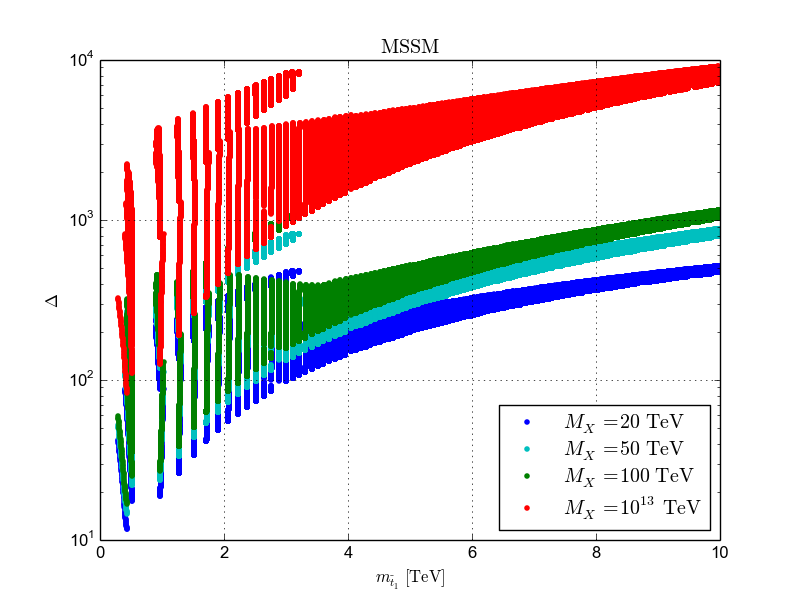
\includegraphics{mssm_stop_tuning.png}}
\resizebox{!}{6cm}{%
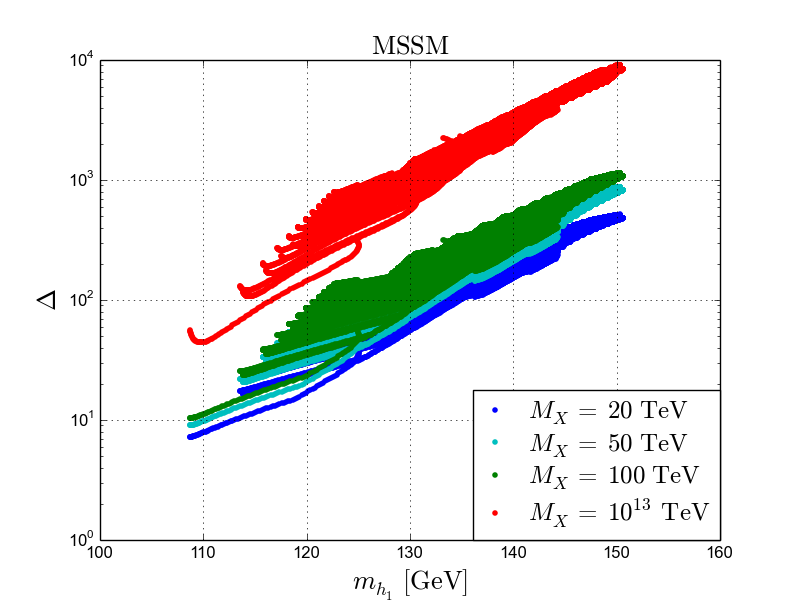
\includegraphics{mssm_higgs_tuning.png}}
\caption{Left panel: Scatter plot of fine tuning in the MSSM as a function of
the lightest stop mass, $m_{\tilde{t}_1}$, for the cut-off scales (from 
bottom to top) $M_X=20$ TeV, $M_X=50$ TeV, $M_X=100$ TeV and $M_X=10^{16}$ GeV. 
Right panel: Scatter plot of fine tuning in the MSSM as a function of
the lightest Higgs mass, $m_{h_1}$, for the cut-off scales (from 
bottom to top) $M_X=20$ TeV, $M_X=50$ TeV, $M_X=100$ TeV and $M_X=10^{16}$ GeV.}
\label{Fig:mssmstoptuning}
\end{center}
\end{figure}
To illustrate this, in the left panel of Fig.~\ref{Fig:mssmstoptuning}
we show the variation in fine tuning when we scan over the stop masses
and mixing, with $500 \textrm{ GeV} \leq m_{Q_3},m_{u_3}\leq
10\textrm{ TeV}$ and $-3810\textrm{ GeV}\leq A_t\leq -20\textrm{
  GeV}$, for $M_X=20$ TeV, $50$ TeV and $100$ TeV.  The remaining
parameters we fix such that at $M_{SUSY}$ they have the values
$\mu=-97.5$ GeV, $B=-84.8$ GeV, $M_1=92.1$ GeV, $M_2=95.9$ GeV,
$M_3=352$ GeV, $A_b=-117.9$ GeV, $A_\tau=-7.8$ GeV, $m_{L_i}=400$ GeV,
$m_{e_i}=204$ GeV, $m_{Q_{1,2}}=438$ GeV, $m_{u_{1,2}}436$ GeV and
$m_{d_i}=438$ GeV ($i=1,2,3$). Although we should stress that making
this choice will lead to a spectrum which is in conflict with the LHC
limits, doing so ensures that fine tuning due to the other parameters
is small, so that we avoid washing out the fine tuning impact of the
stops when the tuning is small\footnote{For models in which the
  spectrum is heavier, when the stop masses are small the fine tuning
  reaches a lower bound imposed by other heavier parameters.} as can
be the case when the stop masses are less than 1 TeV.  Note that the
Higgs mass is also allowed to vary in this scan, as shown in the right
panel of Fig.~\ref{Fig:mssmstoptuning}. This illustrates the tuning
problem which people have been worrying about since the discovery of
the 125 GeV Higgs boson as we see that raising the stop masses is also
pushing up the Higgs mass, meaning that heavier Higgs masses require
more fine tuning.  However for a low value of the UV scale this tuning
is not so severe unless the stops are very heavy, and a 125 GeV Higgs
can be obtained without much tuning in this unrealistic case where we
have minimised other sources of tuning.  On the other hand the tuning
becomes more severe as we increase the cutoff such that for $M_X =
10^{16}$ GeV a lightest stop masses of $1-3$ TeV can result in a fine
tuning of $\approx 100 - 1000$ and the minimum tuning we see consistent
with a $125$ GeV Higgs is $\approx 200$, as shown in
Fig.~\ref{Fig:mssmstoptuning}.

%    - full scatter plots of MSSM and E6SSM, including different
%      M_Z' values

Since the stop mass does not have such a large impact on the fine
tuning when the cutoff scale is very low we can use this to see more
clearly the impact of the $Z^\prime$ mass on fine tuning. To do so we
select a fixed low cutoff of $M_X=20$ TeV and compare the fine tuning
for two different values of the $Z^\prime$ mass. We choose to look at
$M_{Z^\prime}=2.5$ TeV, which is just above the current limits, and
$M_{Z^\prime}=4.5$ TeV, which should be in reach in run II at the LHC
\cite{Godfrey:2013eta} and then compare the fine tuning calculated in
each case to the tuning in the MSSM.  For this, we have performed a
large six dimensional parameter space scan in both the MSSM and
E$_6$SSM, varying those parameters most relevant for the fine tuning
and the Higgs mass.  Therefore the set of parameters which we vary
includes $\mu$, $B$ and $\tan \beta$ for the MSSM, and $\lambda$,
$A_\lambda$ and $\tan \beta$, for the E$_6$SSM, which appear at tree
level in the EWSB conditions of the models. While the RGE contribution
from large stop masses to the fine tuning is small for such a low
cut-off scale, the stop contributions to the effective potential can
play a significant role in reducing the fine tuning.  For this reason it is still important to properly treat the
tuning associated with stop contributions to the one-loop effective
potential, and so we also scan over the soft masses $m_{Q_3}^2$,
$m_{u_3}^2$ and the stop mixing $A_t$.  The relevant parameters and
ranges that were scanned over are summarised in Table
\ref{tab:scanranges}. With the exception of the stop mixing $A_t$ and
the soft trilinear $A_\lambda$, which are logarithmically scanned, all
parameters are linearly scanned.  In addition to this we also repeat
each scan for three different values of $M_2$ to allow more variation
in the chargino masses.

 In this case we now consider realistic scenarios, where the
 parameters that are not scanned over are set to values which keep the
 associated states comfortably above their experimental limits.  So in
 both the MSSM and E$_6$SSM, all other soft scalar masses are set
 to $5$ TeV.  Since we work in the third family approximation, taking
 the first and second generation Yukawa couplings to be zero, we also
 assume their associated soft trilinears vanish. Similarly we take
$A_b=A_\tau=0$ GeV. The $U(1)$ gaugino soft mass $M_1$ was fixed to
 $M_1=300$ GeV, and we fix $M_3=2000$ GeV. Additionally, in the
 E$_6$SSM the $U(1)_N$ gaugino soft mass $M_1'$ is held fixed with
 $M_1'=M_1=300$ GeV, and $\mu^\prime=5$ TeV.  

\begin{table}[h]
\centering
\begin{ruledtabular}
\begin{tabular}{cc}
MSSM & E$_6$SSM \\
\hline
$2 \leq \tan\beta \leq 50$& $2 \leq \tan\beta \leq 50$ \\
$-1\textrm{ TeV } \leq \mu \leq 1 \textrm{ TeV}$ & $-3 \leq \lambda \leq 3$\\
$-1\textrm{ TeV } \leq B \leq 1\textrm{ TeV}$ & $-10\textrm{ TeV } \leq A_\lambda \leq 10\textrm{ TeV}$ \\
$ 200 \textrm{ GeV } \leq m_{Q_3} \leq 2000 \textrm { GeV}$ & $ 200 \textrm{ GeV } \leq m_{Q_3} \leq 2000 \textrm { GeV}$\\
$ 200 \textrm{ GeV } \leq m_{u_3} \leq 2000 \textrm { GeV}$ & $ 200 \textrm{ GeV } \leq m_{u_3} \leq 2000 \textrm { GeV}$\\
$ -10 \textrm{ TeV } \leq A_t \leq 10 \textrm { TeV}$ & $ -10 \textrm{ TeV } \leq A_t \leq 10 \textrm { TeV}$\\
$M_2=100\textrm{ GeV, } 1050\textrm{ GeV, } 2000 \textrm{ GeV}$ & $M_2=100\textrm{ GeV, } 1050\textrm{ GeV, } 2000 \textrm{ GeV}$ \\
\end{tabular}
\end{ruledtabular}
\caption{The parameters scanned over and the ranges of values used in
  the MSSM and the $E_6SSM$ models.}
\label{tab:scanranges}
\end{table}

%   Since the stop mass does not have a large impact on the fine tuning
%   when the cutoff scale is very low we can use this to see more clearly
%   the impact of the $Z^\prime$ mass on fine tuning. To do se we choose a
%   cutoff of  look at the fine tuning for two different
%   values of the $Z^\prime$ mass, $2.5$ TeV, which is just above the
%   current limits and $4.5$ TeV which could be in reach of the LHC run
%   II, and compare these to the MSSM.


%   For this we also fix [what we fix + explain different choices to
%   before and their impact].
\begin{figure}[h]
\begin{center}
\resizebox{!}{10cm}{%
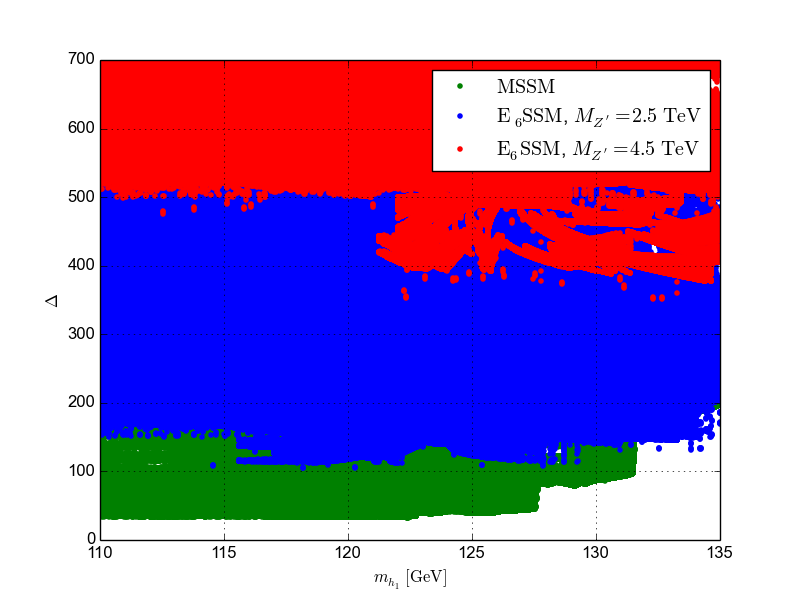
\includegraphics{all_models_tuning_vs_higgs.png}}
\caption{Scatter plot of fine tuning vs lightest Higgs mass for the
  MSSM (green), E$_6$SSM with $M_{Z^\prime} = 2.5$ TeV (blue) and
  E$_6$SSM with $M_{Z^\prime} = 4.5$ TeV (red).}
\label{Fig:e6ssmvsmssm}
\end{center}
\end{figure}
In Fig \ref{Fig:e6ssmvsmssm} results from the scan are plotted showing
the tuning for each case against the lightest Higgs mass.  As expected
the dependence on the Higgs mass is now quite weak, while the minimum
tuning in the model for the E$_6$SSM is increased by the mass of the
$Z^\prime$ boson.  So in the case of a very low cutoff the tuning
required to get a 125 GeV Higgs is not so large.  However the tuning
from the $Z^\prime$ mass appears already at tree level and is
therefore not suppressed when the cutoff scale is low. We find
that in the E$_6$SSM current limits on the mass of the $Z^\prime$
boson imply that the E$_6$SSM fine tuning is at least 100.
Additionally if run II of the LHC pushes the limit on the $Z^\prime$
mass to be above $4.5$ TeV then the fine tuning in the model will be
greater than at least 350.

This demonstrates two important points about these $U(1)$
extensions. Firstly that limits on the $Z^\prime$ mass play an
incredibly important role in constraining natural scenarios in such
models and secondly that the tuning from the $Z^\prime$ limits in
these models depends on less assumptions about SUSY breaking than the
tuning required by the $125$ GeV Higgs measurement which concerns
people in the MSSM.

However we should also acknowledge that there are other limits which
play a similar role.  Chargino limits directly constrain the $\mu$
parameter (or effective $\mu$ parameter in these $U(1)$ extensions).
However the chargino limits from the LHC depend on whether there are
light sleptons or sneutrinos and the mass difference between the
lightest chargino and lightest neutralino.  Current limits placed by
CMS and ATLAS extend up to $m_{\chi^\pm_1} \approx 700-740$ GeV if
there are light sleptons\cite{Khachatryan:2014qwa,Aad:2014nua} with
much weaker bounds if there are no light sleptons or
sneutrinos\footnote{Useful summary plots of these limit may be found
  on the public pages of ATLAS,
  \url{https://atlas.web.cern.ch/Atlas/GROUPS/PHYSICS/CombinedSummaryPlots/SUSY/ATLAS_SUSY_EWSummary/ATLAS_SUSY_EWSummary.png}
  and CMS
  \url{http://cms.web.cern.ch/sites/cms.web.cern.ch/files/styles/large/public/field/image/Image_03_exclusion_Combined.png?itok=8FMBpu_1}.}.




Nonetheless the MSSM the impact of potential chargino mass limits is
shown in Fig.~\ref{Fig:chargino-plot}.  There we see that if the the
full parameter space with $m_{\chi^\pm} < 700$ GeV was excluded the
impact would be to make the tuning in the MSSM with a $20$ TeV cutoff
slightly worse than that of the E$_6$SSM with the same cutoff and a
$Z^\prime$ mass just larger than current limits. In the E$_6$SSM,
while raising the chargino limit can have the same impact in
principle, due to current limits on the $Z^\prime$ mass already
imposing a significant degree of tuning, chargino masses do not make
much of a noticeable change.

\begin{figure}[h]
\begin{center}
\resizebox{!}{10cm}{%
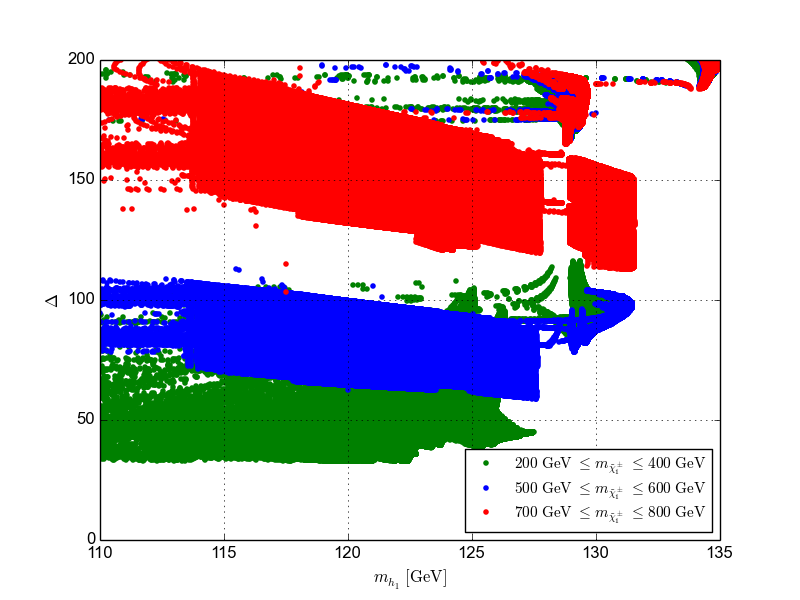
\includegraphics{mssm_chargino_plot.png}}%%
\caption{Scatter plot of fine tuning vs lightest Higgs mass in the MSSM with $m_{\chi^\pm_1} = 200$ GeV shown in green $m_{\chi^\pm_1} = 500$ GeV in blue and $m_{\chi^\pm_1} = 700$ GeV in red.}
\label{Fig:chargino-plot}
\end{center}
\end{figure}

The exact level of tuning from the $Z^\prime$ depends on the charges
of the extra $U(1)$ gauge symmetry it is associated with.  In
Fig.~\ref{Fig:othere6modelsvsmssm} we look at the fine tuning for
other U(1) extensions for the same $Z^\prime$ masses as we did for the
E$_6$SSM.  To simplify the analysis we fix $\tan \beta = 10$, but scan
over the remaining parameters as in Table \ref{tab:scanranges} and fix
the rest to the same values we did in the scan carried out for
Fig.~\ref{Fig:e6ssmvsmssm}.

\begin{figure}
\begin{center}
\resizebox{!}{5cm}{%
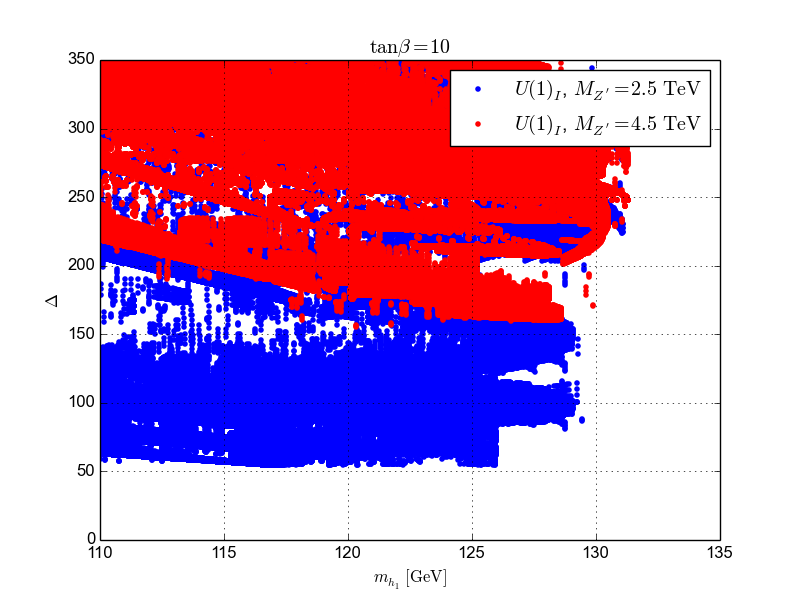
\includegraphics{e6inert_tb10_tuning_vs_higgs.png}}
\resizebox{!}{5cm}{%
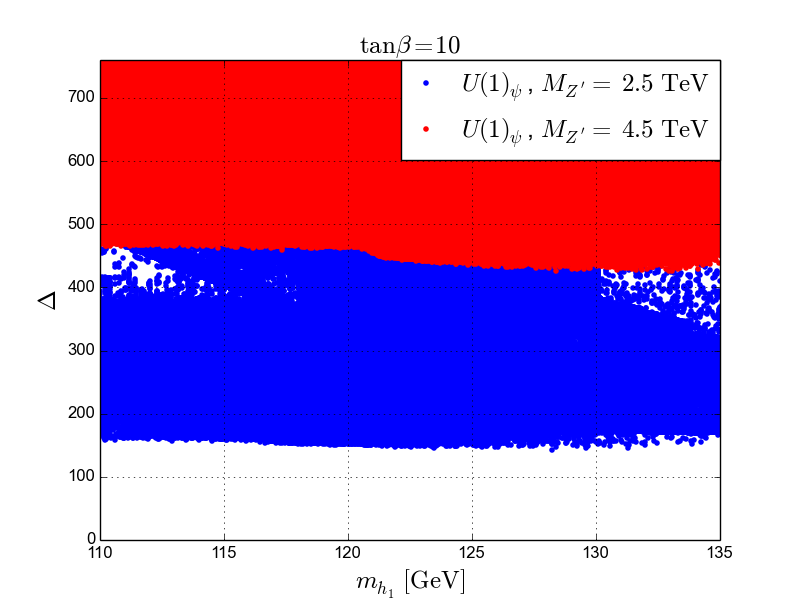
\includegraphics{e6psi_tb10_tuning_vs_higgs.png}}\\
\resizebox{!}{5cm}{%
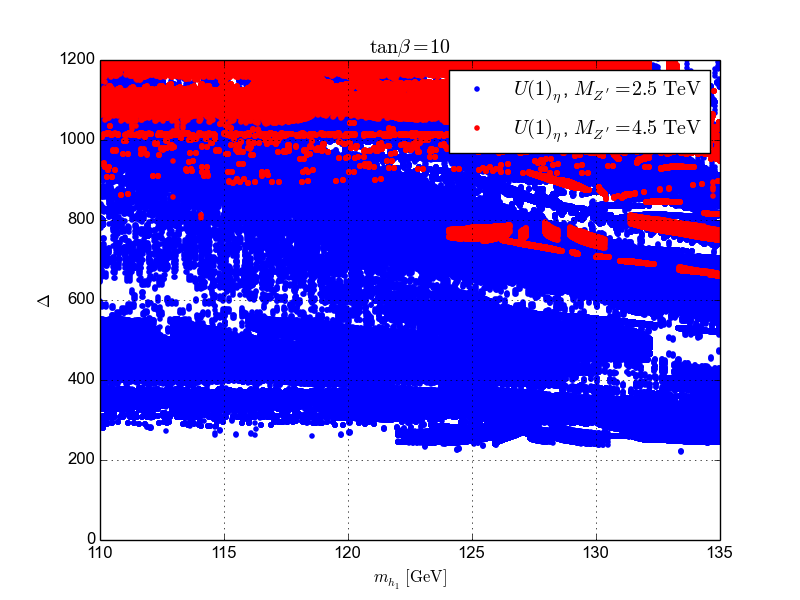
\includegraphics{e6eta_tb10_tuning_vs_higgs.png}}%%
\caption{Scatter plot of fine tuning vs lightest Higgs mass in ... with $M_{Z^\prime} = 2.5$ TeV shown in blue and $M_{Z^\prime} = 4.5$ TeV in red.}
\label{Fig:othere6modelsvsmssm}
\end{center}
\end{figure}

As can be seen in Fig.~\ref{Fig:othere6modelsvsmssm} the severity of the tunings varies quite
a bit.  This is because the charges appear as coefficients in front of
the $Z^\prime$ mass in the EWSB condition.  These charges change the
value of the coefficient $d$ in Eq. (\ref{eq:originalE6MZequation}).
The values of the coefficient $d$ in each model, for $\tan\beta = 10$,
is $\{-0.01, 0.40, 0.50, 0.81 \}$ for $\{U(1)_I, U(1)_N, U(1)_\psi,
U(1)_\eta \}$ and this determines which of the models are most tuned.

Interestingly the coefficient $d$ is very small (and negative) in the
case of the $U(1)_I$.  This allows a dramatic reduction in the fine
tuning from the $U(1)_I$ symmetry.  This is a result of the $H_u$
charge associated with $U(1)_I$ vanishing, which means that the
D-terms to the lightest Higgs which is predominantly $H_u$ at large
$\tan \beta$ are suppressed, making it difficult to raise the Higgs
mass in the same way as happens in the other models and explaining why
heavier Higgs values in this model can't be obtained.  Therefore the fine
tuning behaviour in this model is closer to that of the MSSM, though
the LHC can still constrain the most natural scenarios from just
placing tougher limits on the $Z^\prime$ mass.

Finally we want to emphasise that while in Fig.~\ref{Fig:e6ssmvsmssm}
the E$_6$SSM looks more fine tuned than the MSSM this depends on the
high scale boundary, $M_X$, where the parameters are assumed to be set
by some SUSY breaking mechanism.  Indeed in \cite{Athron:2013ipa} a
constrained version of the E$_6$SSM, with the high scale boundary at
the GUT scale, is considered and there the cE$_6$SSM was found to be
less tuned than the cMSSM. Since a 125 GeV Higgs can be achieved in
the E$_6$SSM with lighter stops, then if the cutoff is large, the
larger stop masses of the MSSM can make that model more fine tuned due
to large RGE effects.

To further illustrate this point we looked at how the tuning varies
with $M_X$ for low tuning benchmarks in the MSSM and E$_6$SSM. These
benchmarks are defined in Table \ref{tab:benchmarks} and the results are shown in
Fig.~\ref{Fig:BMs-varyMX}. Since the behaviour is quite complicated we
now discuss these in detail as it provides some insight into the many
differences in the tuning between the two models.

\begin{table}[h]
\centering
\begin{ruledtabular}
\begin{tabular}{cccc}
& MSSM & E$_6$SSM BM1 & E$_6$SSM BM2 \\
\hline
$\tan\beta(M_Z)$ & 10 & 10 & 10 \\
$s(M_{\mathrm{SUSY}})$ [GeV] & $-$ & 6700 & 6700 \\
$\kappa_{1,2,3}(M_{\mathrm{SUSY}})$ & $-$ & 0.6 & 0.52 \\
$\lambda_{1,2}(M_{\mathrm{SUSY}})$ & $-$ & 0.2 & 0.13 \\
$\mu_{\mathrm{eff}}(M_{\mathrm{SUSY}})$ [GeV] & 689.7 & 1093.3 & 1313.0 \\
$B_{\mathrm{eff}}(M_{\mathrm{SUSY}})$ [GeV] & 345.7 & 3792.7 & 817.8 \\
$A_t(M_{\mathrm{SUSY}})$ [GeV] & -3335.7 & -1100 & -1103.2 \\
$m_{Q3}^2(M_{\mathrm{SUSY}})$ [GeV$^2$] & $4.45\times 10^6$ & $4.50\times 10^5$ & $3.61\times 10^6$ \\
$m_{u3}^2(M_{\mathrm{SUSY}})$ [GeV$^2$] & $4\times 10^6$ & $5.86\times 10^5$ & $2.04\times 10^6$ \\
$M_1(M_{\mathrm{SUSY}})$ [GeV] & 300 & 300 & 173.4 \\
$M_2(M_{\mathrm{SUSY}})$ [GeV] & 2000 & 1050 & 281.4 \\
$M_3(M_{\mathrm{SUSY}})$ [GeV] & 2000 & 2000 & 1200 \\
$M_1^\prime(M_{\mathrm{SUSY}})$ [GeV] & $-$ & 300 & 175.2 \\
\hline
$M_{Z^\prime}$ [GeV] & $-$ & 2473.2 & 2512.7 \\
$m_{h_1}$ [GeV] & 124.3 & 125.0 & 126.2 \\
$m_{\tilde{t}_1}$ [GeV] & 1942.1 & 993.8 & 1665.0 \\
$m_{\tilde{t}_2}$ [GeV] & 2220.1 & 1174.8 & 2094.4 \\
$m_{\tilde{g}}$ [GeV] & 2259.8 & 2290.0 & 1407.4\\
\hline
$\Delta(M_X=20\textrm{ TeV})$ & 157.3 & 165.3 & 402.1 \\
$\Delta(M_X=10^{16}\textrm{ GeV})$ & 1089.0 & 1722.3 & 546.7
\end{tabular}
\end{ruledtabular}
\caption{Parameters and masses for the MSSM point and the E$_6$SSM benchmark points 
BM1 and BM2. For the
E$_6$SSM we define $\mu_{\mathrm{eff}}\equiv \lambda s/\sqrt{2}$ and
$B_{\mathrm{eff}}=A_\lambda$. In BM1 all other (diagonal) soft scalar squared masses not shown above are set to $(5\mathrm{ TeV})^2$, the soft trilinears $A_b$, $A_\tau=0$, $\mu^\prime=5000$ GeV and $B\mu^\prime=5000$ GeV$^2$. In BM2 the parameters not shown above are set to the values obtained by running the cE$_6$SSM point with $m_0=2.2$ TeV, $A_0=500$ GeV, $M_{1/2}=1003$ GeV, $\kappa_{1,2,3}(M_X)=0.1923$, $\lambda(M_X)=0.2646$ to the SUSY scale, and setting $\mu^\prime(M_{\mathrm{SUSY}})=897.9$ GeV and $B\mu^\prime(M_{\mathrm{SUSY}})=-4.2\times10^5$ GeV$^2$.}
\label{tab:benchmarks}
\end{table}

\begin{figure}
\begin{center}
\resizebox{!}{5.5cm}{%
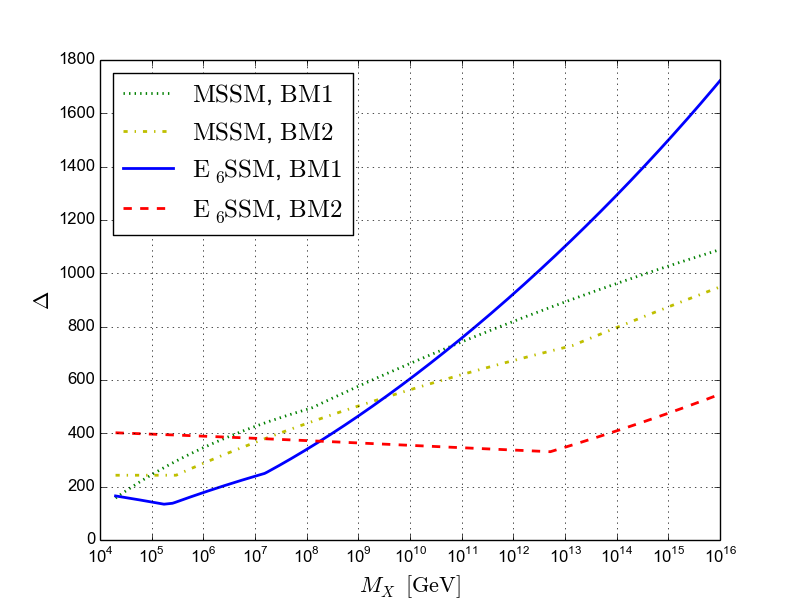
\includegraphics{e6ssm_mssm_cutoff_scan_4_benchmark_points_tuning_vs_cutoff.png} } \\
\resizebox{!}{5.5cm}{%
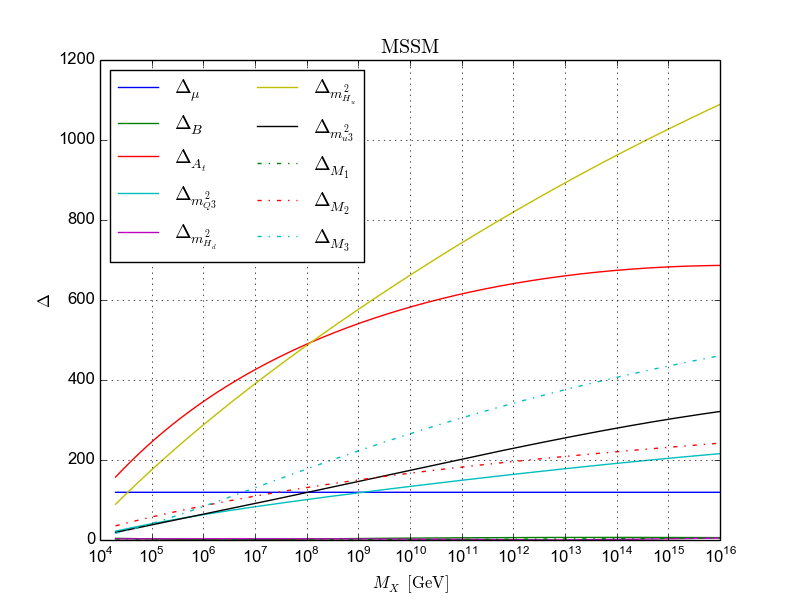
\includegraphics{mssm_cutoff_scan_tb10_fixed_at_ms_all_tuning_data.png}} 
\resizebox{!}{5.5cm}{%
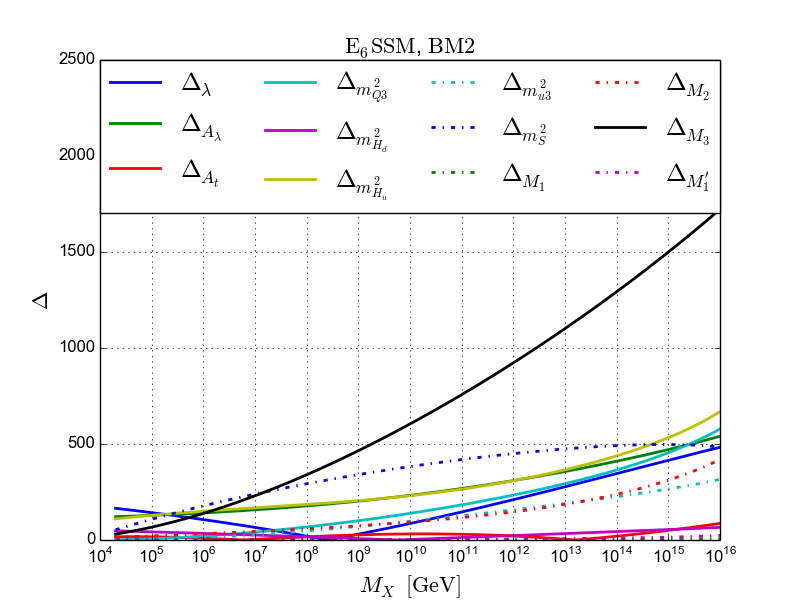
\includegraphics{e6ssm_light_zprime_cutoff_scan_tb10_BM1_all_tuning_data.png}} \\
\resizebox{!}{5.5cm}{%
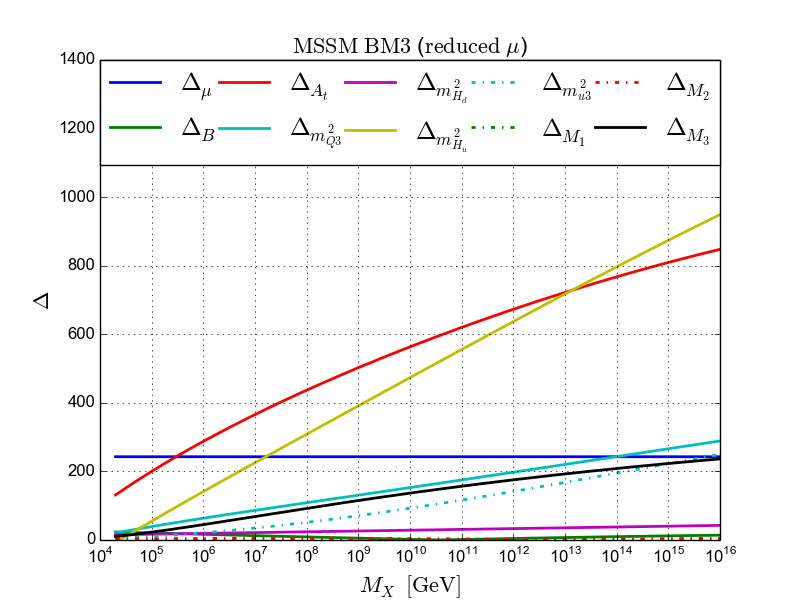
\includegraphics{mssm_cutoff_scan_tb10_fixed_at_ms_BM2_all_tuning_data.png}} 
\resizebox{!}{5.5cm}{%
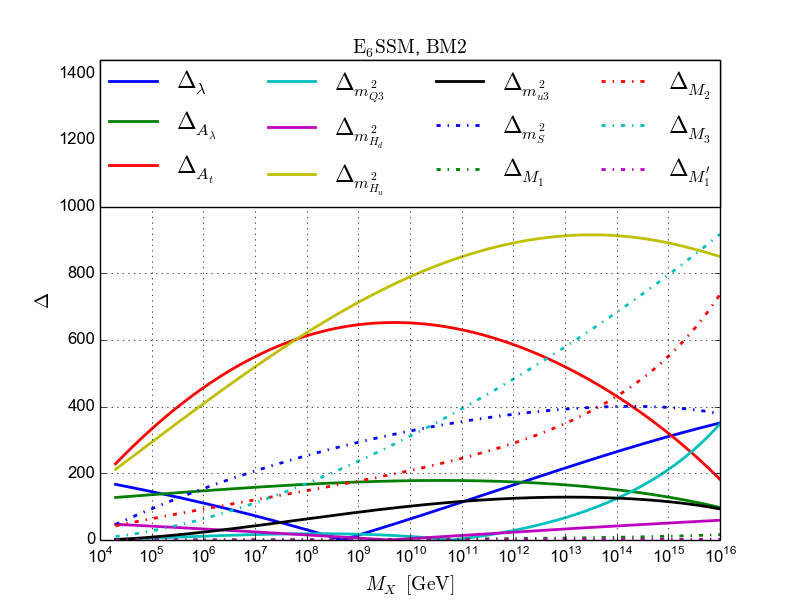
\includegraphics{e6ssm_light_zprime_cutoff_scan_tb10_BM2_all_tuning_data.png}}%%
\caption{{\it Top panel:} Scatter plot of fine tuning vs high scale $M_X$ for the three benchmark points given in Table \ref{tab:benchmarks}.  {\it Middle left panel:}  Individual sensitivities of the MSSM benchmark plotted against the high scale $M_X$ which give an overall tuning shown by the green line in top left panel.  {\it Middle right panel:} Individual sensitivities of E$_6$SSM BM1 plotted against the high scale $M_X$ which give an overall tuning shown by the blue line in top left panel.{\it Bottom right panel:} Individual sensitivities of MSSM BM2 plotted against the high scale $M_X$ which give an overall tuning shown by the red line in top left panel.  {\it Bottom right panel:} Individual sensitivities of E$_6$SSM BM2 plotted against the high scale $M_X$ which give an overall tuning shown by the red line in top left panel.    }
\label{Fig:BMs-varyMX}
\end{center}
\end{figure}

In the top panel one can see that the MSSM BM1 tuning 
steadily climbs as the cutoff scale is increased, as one would expect
when the tuning originates from large soft masses entering from the
RGEs. The panel on the middle left confirms this, showing that the
largest tuning contributions come from $\Delta_{A_t}$ and
$\Delta_{m_{H_u}^2}$ with the former being the larger sensitivity
until $M_X\approx 10^8$ GeV at which point $\Delta_{m_{H_u}^2}$ takes
over, leading to the small kink in overall tuning which can be seen in
the green curve in the top panel. In this case we have chosen a
point with large mixing, which is known to reduce the MSSM tuning.  We
found this does not eliminate the tuning as there is still a strong
sensitivity to $A_t$, but we did find that increasing $A_t$ lead less
fine tuning overall for the points we looked at.  

Comparing the MSSM tunings to the E$_6$SSM tunings one can see that
which point is more fine tuned depends on the scale at which the
parameters are defined.  This illustrates that any statement about
which model is more tuned depends on the high scale boundary, $M_X$.

For E$_6$SSM BM1 the fine tuning is shown by the blue curve in the top
panel of Fig.~\ref{Fig:BMs-varyMX} and the individual sensitivities
are given in the middle right panel. The tuning actually reduces
initially as the cutoff is is increased from $20$ TeV.  This occurs
because the largest sensitivity is initially $\Delta_\lambda$ (shown
in solid blue in the middle right panel).  This contains some terms
proportional to $M_Z^{\prime \, 2}$, which provide the dominant
contribution to this sensitivity at very low $M_X$.  However as $M_X$
is increased contributions from the soft masses become more important
and these actually start to cancel the large contribution to
$\Delta_\lambda$ coming from $M_{Z^\prime}$ until $\Delta_\lambda$
passes through zero.  At the same time though these large soft masses
also cause other sensitivities to grow, in particular $\Delta_{M_3}$.
The fine tuning rises with $M_X$ once $M_X \gtrsim 10^5-10^6$ GeV, but
remains lower than that of the other points, until $M_X \approx 10^8$
GeV.  Eventually the $\Delta_{M_3}$ sensitivity leads to this point
being the most fine tuned of the four shown in
Fig.~\ref{Fig:BMs-varyMX}.

 Although the gluino mass and $M_3(M_{SUSY})$ have similar values to
 those in the MSSM BM1 point, in the E$_6$SSM $M_3(M_X)$ is larger
 due to the altered RGE running from exotic matter\footnote{This
   altered RGE running is a result of the exotic matter introduced to
   keep the extra $U(1)$ anomaly free. }. This is why this E$_6$SSM
 point has the much larger tuning, coming from $\Delta_{M_3}$.


Interestingly other sensitivities are suppressed by this effect since
at the same time larger $M_3$ at higher scales reduces the soft squark
masses at $M_X$.  Therefore the stop mass contributions are
ameliorated, compared to the MSSM, both by allowing lighter stops at
$M_{SUSY}$ and by the modified RGE running.  Nonetheless the stops
still do lead to $\Delta_{m_{H_u}^2}$ increasing with the cutoff
through the usual mechanism \footnote{Wherein $m_{H_u}^2(M_{SUSY})$
  receives a positive contribution to it's mass from $m_{H_u}^2(M_X)$
  and a negative contribution from $m_{Q_3}^2(M_X)$ and
  $m_{U_3}^2(M_X)$, allowing heavy stop masses to cause fine
  tuning. In this case $m_{H_u}^2(M_{SUSY})$ is held fixed so as the
  cutoff increases the values of these soft masses at $M_X$ will be
  larger and there we be a bigger cancellation between them,
  increasing the sensitivity of $M_Z$ to both $m_{H_u}^2$ and the soft
  scalar masses for the stops.}.


By contrast the tuning for E$_6$SSM BM2 is very different, as is shown
in red in the top panel, with the individual sensitivities given in the
bottom right panel. This point was chosen as it had much lighter
gluino mass that is just above the experimental limit of $1.4$ TeV
\cite{Aad:2014lra}.  At $20$ TeV this benchmark is not amongst the
lowest tuned points, since at that scale the tree level tuning from
$M_{Z^\prime}$ dominates.  However the reduction in $M_3$ means that
$\Delta_{M_3}$ is substantially lower and only becomes the dominant
tuning at a much larger scale of $M_X\gtrsim 10^{12}-10^{13}$ GeV,
giving a tuning at $10^{16}$ GeV of $\approx 546$, which is far below
that of the other two benchmark points.

In addition to this, the soft parameters in E$_6$SSM BM2 follow a pattern similar to that found in the constrained
model. With the exception of the parameters $m_{Q3}^2$, 
$m_{u3}^2$, $m_{H_d}^2$, $m_{H_u}^2$, and $M_3$, the values of which are given in Table \ref{tab:benchmarks}, 
the soft masses at the SUSY scale correspond to the values that result in the cE$_6$SSM with $m_0=2.2$ TeV, 
$M_{1/2}=1003$ GeV, $A_0=500$ GeV, $\kappa_{1,2,3}(M_X)=0.1923$, $\lambda(M_X)=0.2646$ and
$\lambda_{1,2}(M_X)=0.1$. This leads to a significant reduction in the contributions to the RG running of $m_{H_u}^2$ and $m_{Q3}^2$ coming from terms of the form $g_1^2\Sigma_1$ and, to a lesser extent, $g_1'^2\Sigma_1'$. Here we define (see also Eq.~(\ref{}))
\begin{align*}
\Sigma_1&=\sum_{i=1}^3\left ( m_{Qi}^2-2m_{ui}^2+m_{di}^2+m_{ei}^2-m_{Li}^2+m_{H_{ui}}^2-m_{H_{di}}^2+m_{\overline{D}_i}^2-m_{Di}^2\right )-m_{H'}^2+m_{\overline{H'}}^2,\\
\Sigma_1'&=\sum_{i=1}^3\left ( 6m_{Qi}^2+3m_{ui}^2+6m_{di}^2+m_{ei}^2+4m_{Li}^2-4m_{H_{ui}}^2-6m_{H_{di}}^2+5m_{Si}^2-9m_{\overline{D}_i}^2-6m_{Di}^2\right )\\
&\quad{}+4m_{H'}^2-4m_{\overline{H'}}^2.
\end{align*}
In the unconstrained case, this contribution acts to drive up the values of $m_{Q3}^2$ and $m_{H_u}^2$, and thus the associated tuning sensitivities, at the input scale $M_X$. In the case of E$_6$SSM BM2, on the other hand, the reduced splitting between the soft masses leads to a much smaller contribution from these terms. Together with the reduction in $M_3$ described above, this allows to maintain the observed low fine tuning at very large values of $M_X$.

MSSM benchmark BM2 (yellow in top panel, individual sensitivities in bottom left panel) was designed to be similar to E$_6$SSM BM2, for a reasonable comparison.  However from the individual sensitivities one can see that the behaviour is quite similar to MSSM BM1, though in this case the $\Delta_{m_{H_u}^2}$ becomes the largest tuning at a higher $M_X$ and does not reach such large values, since more of the tuning is from the mixing in this case.

\section{\label{sec:conclusion}Conclusions}

Prior to stringent experimental constraints on the mass of the
lightest Higgs boson and squarks in supersymmetric models, a simple
picture of a natural SUSY model emerged from theoretical reasoning,
with soft masses set to similar values at the GUT scale through local
gravity interactions with the hidden sector.  Through the use of
renormalisation group running one can then see that at the EW scale
the stops and soft Higgs masses (which appear directly in the EWSB
conditions) should appear in the the EWSB condition for $M_Z$ and
therefore it was expected that these masses should not be much bigger
than $100$ GeV.  However to disturb this elegant picture first LEP
placed constraints on the Higgs mass, requiring it to be above 114.4
GeV \cite{Barate:2003sz,Schael:2006cr}, which already introduced significant tuning for
constrained models, since heavy stops are required to raised the
lightest Higgs mass above it's tree level bound. Recently this problem
got much worse since the LHC measured the Higgs to be around $125$
GeV.

$U(1)$ extensions motivated by the $\mu$-problem, $E_6$ GUT theories
and the connection to string theory contain both $F-$ and $D-$ term
contributions to the light Higgs mass which can raise the tree level
mass, evading the need for large radiative corrections to increase it.
However such models come with their own fine tuning problem, where the
$Z^\prime$ mass appears in the EWSB condition for $M_Z$ at tree level.
While in a previous study of the constrained E$_6$SSM it was found
that the tuning is less severe than the MSSM, it was still significant.


In light of such difficulties it is worth considering whether the
simple picture which emerged is wrong in some way and if there are
other possibilities that allow naturalness.  Or to phrase this in a
more challenging manner are there ways to constrain the naturalness of
these models that do not rely upon assumptions about how SUSY is
broken?

We have investigated this question here in the context of the MSSM and
U(1) extensions.  Since the RG evolution links the soft masses
together and causes these problems from stop and gluino masses the
most conservative approach to placing naturalness limits is to choose
a low cutoff. We find that in the MSSM the most direct way to
constrain naturalness of the model, without making assumptions about
the SUSY breaking scale is through limits on the chargino
masses. Current LHC limits on charginos are not model independent and
thereby leave many gaps where on can have light charginos.

% DH:: I've given the minimum overall tunings for each, would it be
% better to give the minimum for a 125 GeV Higgs (which is
% ~38 for the MSSM, at a Higgs mass of 125.04 GeV, \tan\beta = 50,
% vs. ~122 for a 2.5 TeV Z' and 393 for a 4.5 TeV Z' with m_h = 125.5 GeV
% (this increases to ~416 for a 125 GeV Higgs exactly)
In contrast we find that in $U(1)$ extensions of the MSSM there is an
additional way to constrain the naturalness of the models, which is
through the $Z^\prime$ mass limit.  We find when we impose a low
cutoff of $20$ TeV for setting the soft masses, the lowest tuning in
the E$_6$SSM is compatible with a $Z^\prime$ mass of $2.5$ TeV was
$\Delta \approx 112$, while if the LHC run II can place a limit of
$4.5$ TeV on $M_Z^\prime$ then the tuning would be approximately $380$.
By comparison the current situation in the MSSM only requires a tuning
of around $33$. This should be interpreted as saying that in
the most conservative limits one can place on naturalness on these
models, the tuning in the E$_6$SSM is worse.  However if there are no
charginos below $700$ GeV then the situation in the two models would
be the same.

This should also be contrasted with what happens as we raise the high
scale boundary, $M_X$.  We showed that for benchmark points that which
one is more tuned depends very strongly on $M_X$.  The E$_6$SSM tuning
is sufficiently complicated by the interplay of these different
sources of tension in the EWSB conditions that a small reduction in
fine tuning can even occur for a moderate increase in $M_X$.  However
as $M_X$ increases towards the scale where the gauge couplings unify,
the familiar tunings do dominate, though with tunings from the Gluino
mass appearing to be more significant relative to those from soft
scalar masses.  


We also looked at the tuning in different $U(1)$ extensions for
fixed $\tan \beta = 10$.  We found that in all cases the fine tuning
was much worse for the larger $Z^\prime$ mass, further emphasising
the importance they play in these $U(1)$ extensions.  Interestingly
the actual level in tuning varied quite a bit between these models
with the $U(1)_I$ model showing the least tuning due to the vanishing
charge of the $H_u$ state. This model is quite interesting in the
sense that it provides a solution to the $\mu$-problem while avoiding
the large tuning (with current limits) from the $Z^\prime$
mass. However one should remember we are looking at conservative limits
on naturalness here and there is no solution to the usual tuning from
the large stops needed to get a $125$ GeV Higgs in this model.  In any
case future LHC limits on the $Z^\prime$ mass would be especially
interesting for this case as they would significantly raise the
minimum level of tuning which can be obtained.


 
% Our conclusions: at low scales stops are not a big contributor,
% Z' causes a significant fine tuning in the E6SSM (dominant -> lower
% bound), chargino bounds will be important for fine tuning in the MSSM
% but not as much for the E6SSM, and possibly discuss different U(1)' charges.
\appendix
\section{\label{app:masterformula}Fine Tuning Master Formula}
% Tree level master formula for the E6SSM
To write down the tree level master formula, it is convenient to define the quantities
\begin{equation}
z_i =\epsilon_{ijk} \frac{\partial f_j}{\partial s}\frac{\partial f_k}{\partial \tan\beta}
\label{eq:masterformulacoefficients}
\end{equation}
with $f_1,f_2,f_3$ as given in Eq. (\ref{eq:E6EWSBConditions}). The relevant partial derivatives are
\ba
\frac{\partial f_1}{\partial \tan\beta}&=&-\frac{2M_Z}{\bar{g}}\,\cos^2\beta\left \{ \frac{\lambda A_\lambda s}{\sqrt{2}}\,\cos\beta+\sin\beta \left [ m_{H_d}^2+\frac{s^2}{2}\left ( \lambda^2+g_1'^2\tilde{Q}_1\tilde{Q}_S \right )\right.\right.\nonumber\\
&&\left.\left.+M_Z^2\left ( \frac{5}{2}-\frac{4\lambda^2}{\bar{g}^2}-\frac{4g_1'^2}{\bar{g}^2}\tilde{Q}_1\tilde{Q}_2+\frac{6g_1'^2}{\bar{g}^2}\tilde{Q}_1^2\right )\right ]+3M_Z^2\,\sin^3\beta\left [ \frac{2\lambda^2}{\bar{g}^2}-1\right.\right.\nonumber\\
&&\left.\left.+\frac{2g_1'^2}{\bar{g}^2}\left ( \tilde{Q}_1\tilde{Q}_2-\tilde{Q}_1^2\right )\right ]\right \},\nonumber\\
\frac{\partial f_1}{\partial s}&=&\frac{2M_Z}{\bar{g}}\left [ s\left ( \lambda^2+g_1'^2\tilde{Q}_1\tilde{Q}_S\right )\,\cos\beta-\frac{\lambda A_\lambda}{\sqrt{2}}\,\sin\beta \right ],\nonumber\\
\frac{\partial f_2}{\partial \tan\beta}&=&\frac{2M_Z}{\bar{g}}\,\cos^2\beta\left \{ \frac{\lambda A_\lambda s}{\sqrt{2}}\,\sin\beta+\cos\beta\left [ m_{H_u}^2+\frac{s^2}{2}\left ( \lambda^2+g_1'^2\tilde{Q}_2\tilde{Q}_S \right )\right.\right.\nonumber\\
&&\left.+M_Z^2\left ( \frac{5}{2}-\frac{4\lambda^2}{\bar{g}^2}-\frac{4g_1'^2}{\bar{g}^2}\tilde{Q}_1\tilde{Q}_2+\frac{6g_1'^2}{\bar{g}^2}\tilde{Q}_2^2\right )\right ]+3M_Z^2\,\cos^3\beta \left [ \frac{2\lambda^2}{\bar{g}^2}-1\right.\nonumber\\
&&\left.\left.+\frac{2g_1'^2}{\bar{g}^2}\left ( \tilde{Q}_1\tilde{Q}_2-\tilde{Q}_2^2\right )\right ]\right \},\nonumber\\
\frac{\partial f_2}{\partial s}&=&\frac{2M_Z}{\bar{g}}\left [ s\left ( \lambda^2+g_1'^2\tilde{Q}_2\tilde{Q}_S\right )\,\sin\beta-\frac{\lambda A_\lambda}{\sqrt{2}}\,\cos\beta\right ],\nonumber\\
\frac{\partial f_3}{\partial \tan\beta}&=&\frac{2M_Z^2}{\bar{g}^2}\,\cos^2\beta\left [ g_1'^2\tilde{Q}_Ss\left ( \tilde{Q}_2-\tilde{Q}_1\right )\,\sin 2\beta-\sqrt{2}\lambda A_\lambda\,\cos 2\beta\right ],\nonumber\\
\frac{\partial f_3}{\partial s}&=&m_S^2+\frac{2\lambda^2M_Z^2}{\bar{g}^2}+\frac{g_1'^2}{2}\tilde{Q}_S\left [\frac{4M_Z^2}{\bar{g}^2}\left ( \tilde{Q}_1\,\cos^2\beta+\tilde{Q}_2\,\sin^2\beta\right ) +3\tilde{Q}_S s^2\right ].\nonumber
\ea
For a running parameter $q$ appearing in the tree level EWSB conditions, the corresponding contribution to the sensitivity coefficient can then be written 
\be
\tilde{\Delta}_q=z_1\frac{\partial f_1}{\partial q}+z_2\frac{\partial f_2}{\partial q}+z_3\frac{\partial f_3}{\partial q}.
\label{eq:tuningContribution}
\ee
It is straightforward to compute the appropriate derivatives directly from the EWSB conditions (\ref{eq:E6EWSBConditions}). Similarly, the quantity $C$ appearing in Eq. (\ref{eq:E6masterformula}) is given by
\be
C=\frac{1}{2}\left ( z_1\frac{\partial f_1}{\partial M_Z}+z_2\frac{\partial f_2}{\partial M_Z}+z_3\frac{\partial f_3}{\partial M_Z}\right ),
\label{eq:tuningDenominator}
\ee
with 
\ba
\frac{\partial f_1}{\partial M_Z}&=&\frac{2}{\bar{g}}\,\cos\beta\left ( m_{H_d}^2+\frac{\lambda^2s^2}{2}+\frac{g_1'^2}{2}\tilde{Q}_1\tilde{Q}_Ss^2+\frac{6g_1'^2}{\bar{g}^2}\tilde{Q}_1^2M_Z^2\right )-\sqrt{2}\frac{\lambda A_\lambda s}{\bar{g}}\,\sin\beta\nonumber \\
&&+\frac{3M_Z^2}{\bar{g}}\,\cos\beta\,\cos 2\beta+\frac{6}{\bar{g}^3}M_Z^2\,\sin\beta\,\sin 2\beta\left [ \lambda^2+g_1'^2\left(\tilde{Q}_1\tilde{Q}_2-\tilde{Q}_1^2\right )\right ],\nonumber\\
\frac{\partial f_2}{\partial M_Z}&=&\frac{2}{\bar{g}}\,\sin\beta\left ( m_{H_u}^2+\frac{\lambda^2s^2}{2}+\frac{g_1'^2}{2}\tilde{Q}_2\tilde{Q}_Ss^2+\frac{6g_1'^2}{\bar{g}^2}\tilde{Q}_2^2M_Z^2\right )-\sqrt{2}\frac{\lambda A_\lambda s}{\bar{g}}\,\cos\beta \nonumber\\
&&-\frac{3M_Z^2}{\bar{g}}\,\sin\beta\,\cos 2\beta+\frac{6}{\bar{g}^3}M_Z^2\,\cos\beta\,\sin 2\beta\left [ \lambda^2+g_1'^2\left ( \tilde{Q}_1\tilde{Q}_2-\tilde{Q_2}^2\right )\right ],\nonumber \\
\frac{\partial f_3}{\partial M_Z}&=&\frac{4M_Z}{\bar{g}^2}\left [ \lambda^2s-\frac{\lambda A_\lambda}{\sqrt{2}}\,\sin 2\beta+g_1'^2\tilde{Q}_Ss\left ( \tilde{Q}_1\,\cos^2\beta+\tilde{Q}_2\,\sin^2\beta \right )\right ].\nonumber
\ea
\section{\label{app:rges}RGE Contributions}
% List the derivatives needed in the Taylor series approximation
% to the RGE solutions.
Provided that one does not run over too large a range of scales, the
solutions to the RG equations for a model can be reasonably well
approximated by a Taylor series, Eq. (\ref{eq:rgeapproxsoln}).  For a
parameter $p$, this reads
\begin{equation*}
q(Q)=q(M_X)+\frac{t}{16\pi^2}\left ( \beta_q^{(1)}+\frac{\beta_q^{(2)}}{16\pi^2}\right )+\frac{t^2}{(16\pi^2)^2}b_q^{(2)}(M_X),
\end{equation*}
where we have for convenience defined
\begin{equation*}
b_q^{(2)}(M_X)=\frac{1}{2!}\left . \sum_{q_k}\beta_{q_k}^{(1)}\frac{\partial \beta_q}{\partial q_k}\right |_{M_X}.
\end{equation*}
We have constructed the necessary series solutions in both the MSSM
and the $U(1)$ extended models. Due to the smallness of the first and
second generation Yukawa couplings, we neglect them in our
calculations. The corresponding soft SUSY breaking trilinears are
likewise omitted. Additionally, all soft mass matrices are assumed
diagonal, and the gaugino masses are taken to be real.\\ \\ In the
MSSM, the relevant parameters for the fine tuning calculation are
$\mu$, $B$, $m_{H_u}^2$, $m_{H_d}^2$ at tree level. The one- and
two-loop RGEs for these parameters may be found in
\cite{Martin:1993zk}. The corresponding $O(t^2)$ contributions are
\begin{subequations}\label{eq:MSSMTreeLevelCoeffs}
\begin{align}
b_\mu^{(2)}&=\frac{\mu}{2}\Bigg [ 45y_t^4+45y_b^4+9y_\tau^2+30y_t^2y_b^2+6y_t^2y_\tau^2+18y_b^2y_\tau^2-32g_3^2(y_t^2+y_b^2)\nonumber\\
&\quad{}-12g_2^2(3y_t^2+3y_b^2+y_\tau^2)-\frac{4}{5}g_1^2(11y_t^2+8y_b^2+6y_\tau^2)+3g_2^4-\frac{189}{25}g_1^4+\frac{18}{5}g_1^2g_2^2\Bigg ],\label{eq:MSSMmub2}\\
b_B^{(2)}&=72y_t^4A_t+72y_b^4A_b+16y_\tau^4A_\tau+12y_t^2y_b^2(A_t+A_b)+12y_\tau^2y_b^2(A_b+A_\tau)\nonumber\\
&\quad{}-32g_3^2y_t^2(A_t-M_3)-32g_3^2y_b^2(A_b-M_3)\nonumber\\
&\quad{}-18g_2^2y_t^2(A_t-M_2)-18g_2^2y_b^2(A_b-M_2)-6g_2^2y_\tau^2(A_\tau-M_2)\nonumber\\
&\quad{}-\frac{26}{5}g_1^2y_t^2(A_t-M_1)-\frac{14}{5}g_1^2y_b^2(A_b-M_1)-\frac{18}{5}g_1^2y_\tau^2(A_\tau-M_1)\nonumber\\
&\quad{}+12g_2^4M_2+\frac{396}{25}g_1^4M_1,\label{eq:MSSMBb2}\\
b_{m_{H_d}^2}^{(2)}&=72y_b^4\left ( m_{H_d}^2+m_{Q3}^2+m_{d3}^2+2A_b^2\right )\nonumber\\
&\quad{}+6y_t^2y_b^2\left ( m_{H_u}^2+m_{H_d}^2+2m_{Q3}^2+m_{u3}^2+m_{d3}^2+(A_t+A_b)^2\right )\nonumber\\
&\quad{}+12y_\tau^2y_b^2\left ( 2m_{H_d}^2+m_{Q3}^2+m_{d3}^2+m_{L3}^2+m_{e3}^2+(A_\tau+A_b)^2\right )\nonumber\\
&\quad{}+16y_\tau^4\left ( m_{H_d}^2+m_{L3}^2+m_{e3}^2+2A_\tau^2\right )\nonumber\\
&\quad{}-32g_3^2y_b^2\left ( m_{H_d}^2+m_{Q3}^2+m_{d3}^2+A_b^2-2M_3A_b+2M_3^2\right )\nonumber\\
&\quad{}-18g_2^2y_b^2\left ( m_{H_d}^2+m_{Q3}^2+m_{d3}^2+A_b^2-2M_2A_b+2M_2^2\right )\nonumber\\
&\quad{}-6g_2^2y_\tau^2\left ( m_{H_d}^2+m_{L3}^2+m_{e3}^2+A_\tau^2-2M_2A_\tau+2M_2^2\right )\nonumber\\
&\quad{}-\frac{14}{5}g_1^2y_b^2\left ( m_{H_d}^2+m_{Q3}^2+m_{d3}^2+A_b^2-2M_1A_b+2M_1^2\right )\nonumber\\
&\quad{}-\frac{18}{5}g_1^2y_\tau^2\left ( m_{H_d}^2+m_{L3}^2+m_{e3}^2+A_\tau^2-2M_1A_\tau+2M_1^2\right )\nonumber\\
&\quad{}-18g_2^4M_2^2-\frac{198}{25}g_1^4\left ( \mathcal{S}+3M_1^2\right ),\label{eq:MSSMmHd2b2}\\
b_{m_{H_u}^2}^{(2)}&=72y_t^4\left ( m_{H_u}^2+m_{Q3}^2+m_{u3}^2+2A_t^2\right )\nonumber\\
&\quad{}+6y_t^2y_b^2\left ( m_{H_u}^2+m_{H_d}^2+2m_{Q3}^2+m_{u3}^2+m_{d3}^2+(A_t+A_b)^2\right )\nonumber\\
&\quad{}-32g_3^2y_t^2\left ( m_{H_u}^2+m_{Q3}^2+m_{u3}^2+A_t^2-2A_tM_3+2M_3^2\right )\nonumber\\
&\quad{}-18g_2^2y_t^2\left ( m_{H_u}^2+m_{Q3}^2+m_{u3}^2+A_t^2-2A_tM_2+2M_2^2\right )\nonumber\\
&\quad{}-\frac{26}{5}g_1^2y_t^2\left ( m_{H_u}^2+m_{Q3}^2+m_{u3}^2+A_t^2-2A_tM_1+2M_1^2\right )\nonumber\\
&\quad{}+\frac{198}{25}g_1^4\left ( \mathcal{S}-3M_1^2\right )-18g_2^4M_2^2.\label{eq:MSSMmHu2b2}
\end{align}
\end{subequations}
In these expressions the quantity $\mathcal{S}$ is defined by
\begin{equation}\label{eq:MSSMgaugeBetaContribution}
\mathcal{S}=m_{H_u}^2-m_{H_d}^2+\sum_{i=1}^3\left ( m_{Qi}^2-m_{Li}^2-2m_{ui}^2+m_{di}^2+m_{ei}^2\right ).
\end{equation}
If in addition the one-loop contributions to the effective potential
from top and stop loops are included, it is also necessary to
construct the expansions for $m_{Q3}^2$, $m_{u3}^2$ and $A_t$. The
coefficients read
\begin{subequations}\label{eq:MSSMsEffPotCoeffs}
\begin{align}
b_{m_{Q3}^2}^{(2)}&=24y_t^4\left ( m_{H_u}^2+m_{Q3}^2+m_{u3}^2+2A_t^2\right )+24y_b^4\left ( m_{H_d}^2+m_{Q3}^2+m_{d3}^2+2A_b^2\right )\nonumber\\
&\quad{}+4y_t^2y_b^2\left ( m_{H_u}^2+m_{H_d}^2+2m_{Q3}^2+m_{u3}^2+m_{d3}^2+(A_t+A_b)^2\right )\nonumber\\
&\quad{}+2y_b^2y_\tau^2\left ( 2m_{H_d}^2+m_{Q3}^2+m_{L3}^2+m_{d3}^2+m_{e3}^2+(A_b+A_\tau)^2\right )\nonumber\\
&\quad{}-\frac{32}{3}g_3^2y_t^2\left ( m_{H_u}^2+m_{Q3}^2+m_{u3}^2+A_t^2-2M_3A_t+2M_3^2\right )\nonumber\\
&\quad{}-\frac{32}{3}g_3^2y_b^2\left ( m_{H_d}^2+m_{Q3}^2+m_{d3}^2+A_b^2-2M_3A_b+2M_3^2\right )\nonumber\\
&\quad{}-6g_2^2y_t^2\left ( m_{H_u}^2+m_{Q3}^2+m_{u3}^2+A_t^2-2M_2A_t+2M_2^2\right )\nonumber\\
&\quad{}-6g_2^2y_b^2\left ( m_{H_d}^2+m_{Q3}^2+m_{d3}^2+A_b^2-2M_2A_b+2M_2^2\right )\nonumber\\
&\quad{}-\frac{26}{15}g_1^2y_t^2\left ( m_{H_u}^2+m_{Q3}^2+m_{u3}^2+A_t^2-2M_1A_t+2M_1^2\right )\nonumber\\
&\quad{}-\frac{14}{15}g_1^2y_b^2\left ( m_{H_d}^2+m_{Q3}^2+m_{d3}^2+A_b^2-2M_1A_b+2M_1^2\right )\nonumber\\
&\quad{}+96g_3^4M_3^2-18g_2^4M_2^2+\frac{66}{25}g_1^4(\mathcal{S}-M_1^2),\label{eq:MSSMmQ32b2}\\
b_{m_{u3}^2}^{(2)}&=48y_t^4\left ( m_{H_u}^2+m_{Q3}^2+m_{u3}^2+2A_t^2\right )\nonumber\\
&\quad{}+4y_t^2y_b^2\left ( m_{H_u}^2+m_{H_d}^2+2m_{Q3}^2+m_{u3}^2+m_{d3}^2+(A_t+A_b)^2\right )\nonumber\\
&\quad{}-\frac{64}{3}g_3^2y_t^2\left ( m_{H_u}^2+m_{Q3}^2+m_{u3}^2+A_t^2-2M_3A_t+2M_3^2\right )\nonumber\\
&\quad{}-12g_2^2y_t^2\left ( m_{H_u}^2+m_{Q3}^2+m_{u3}^2+A_t^2-2M_2A_t+2M_2^2\right )\nonumber\\
&\quad{}-\frac{52}{15}g_1^2y_t^2\left ( m_{H_u}^2+m_{Q3}^2+m_{u3}^2+A_t^2-2M_1A_t+2M_1^2\right )\nonumber\\
&\quad{}+96g_3^4M_3^2-\frac{264}{25}g_1^4\left ( \mathcal{S}+4M_1^2\right ),\label{eq:MSSMmu32b2}\\
b_{A_t}^{(2)}&=144y_t^4A_t+24y_b^4A_b+14y_t^2y_b^2(A_t+A_b)+2y_b^2y_\tau^2(A_b+A_\tau)\nonumber\\
&\quad{}-64g_3^2y_t^2(A_t-M_3)-36g_2^2y_t^2(A_t-M_2)-\frac{52}{5}g_1^2y_t^2(A_t-M_1)\nonumber\\
&\quad{}-\frac{32}{3}g_3^2y_b^2(A_b-M_3)-6g_2^2y_b^2(A_b-M_2)-\frac{14}{15}g_1^2y_b^2(A_b-M_1)\nonumber\\
&\quad{}-64g_3^4M_3+12g_2^4M_2+\frac{572}{25}g_1^4M_1.\label{eq:MSSMAtb2}
\end{align}
\end{subequations}
Similarly we can obtain the two-loop $\beta$ functions and
coefficients $b_p^{(2)}$ for a general set of $U(1)'$
charges. Two-loop RGEs for the gauge and Yukawa couplings, gaugino
masses and soft trilinears, along with the one-loop RGEs for the soft
scalar masses, were given in \cite{Athron:2009bs} for the particular
case of the E$_6$SSM. At tree level in the EWSB conditions the
parameters that must be considered are $\lambda$, $A_\lambda$,
$m_{H_u}^2$, $m_{H_d}^2$, $m_S^2$ and $g_1$, $g_2$ and $g_1'$. The
one- and two-loop contributions to the $\beta$ function for $\lambda$
are
\begin{subequations}\label{eq:USSMLambdaBetas}
\begin{align}
\beta_\lambda^{(1)}&=\lambda  \left[2\lambda ^2+2 \Sigma_\lambda +3 \Sigma_\kappa +3 y_t^2+3 y_b^2+y_{\tau }^2-3 g_2^2-\frac{3}{5} g_1^2 -2 \left ( \tilde{Q}_1^2 + \tilde{Q}_2^2 + \tilde{Q}_S^2\right )g_1'^2 \right],\label{eq:USSMLambdaBetaOneLoop}\\
\beta_\lambda^{(2)}&=\lambda \bigg \{ -2\lambda^2\left ( \lambda^2+2\Sigma_\lambda+3\Sigma_\kappa\right )-4\Pi_\lambda-6\Pi_\kappa-3\lambda^2\left ( 3y_t^2+3y_b^2+y_\tau^2\right ) \nonumber\\
&{} -3\left ( 3y_t^4+3y_b^4+2y_t^2y_b^2+y_\tau^2 \right )+6g_2^2\Sigma_\lambda+g_1^2\left ( \frac{4}{5}y_t^2-\frac{2}{5}y_b^2+\frac{6}{5}y_\tau^2+\frac{4}{5}\Sigma_\kappa +\frac{6}{5}\Sigma_\lambda\right )\nonumber\\
&{}\left.+g_1'^2\left [ 4\tilde{Q}_S^2\lambda^2 -6\left ( \tilde{Q}_2^2-\tilde{Q}_Q^2-\tilde{Q}_u^2\right )y_t^2-6\left ( \tilde{Q}_1^2-\tilde{Q}_Q^2-\tilde{Q}_d^2\right )y_b^2 \right.\right.\nonumber\\
&{}\left.-2\left ( \tilde{Q}_1^2-\tilde{Q}_L^2-\tilde{Q}_e^2\right )y_\tau^2-6\left ( \tilde{Q}_S^2-\tilde{Q}_D^2-\tilde{Q}_{\overline{D}}^2 \right )\Sigma_\kappa-4\left ( \tilde{Q}_S^2-\tilde{Q}_1^2-\tilde{Q}_2^2\right )\Sigma_\lambda\right ]\nonumber\\
&{}+16g_3^2\left ( y_t^2+y_b^2+\Sigma_\kappa\right ) +\frac{33}{2}g_2^4+\frac{297}{50}g_1^4+2g_1'^4\left [ 2\tilde{Q}_1^4+2\tilde{Q}_2^4+2\tilde{Q}_S^4+\left ( \tilde{Q}_1^2+\tilde{Q}_2^2+\tilde{Q}_S^2\right )\Sigma_{\tilde{Q}}\right ]\nonumber\\
&{}+\frac{9}{5}g_1^2g_2^2+6g_1'^2g_2^2\left ( \tilde{Q}_1^2+\tilde{Q}_2^2\right )+\frac{6}{5}g_1^2g_1'^2\left [\tilde{Q}_1^2+\tilde{Q}_2^2+\left ( \tilde{Q}_2-\tilde{Q}_1\right )\Sigma_{\tilde{Q}}^Y\right ]\bigg \},\label{eq:USSMLambdaBetaTwoLoop}
\end{align}
\end{subequations}
where
\begin{equation*}
\Sigma_\lambda=\lambda_1^2+\lambda_2^2+\lambda_3^2, \qquad \Sigma_\kappa=\kappa_1^2+\kappa_2^2+\kappa_3^2.
\end{equation*}
Additionally, in order to keep our expressions compact we also use the notation
\begin{align*}
\Sigma_{\tilde{Q}}=\sum_i \tilde{Q}_i^2, \qquad \Pi_{\tilde{Q}}=\sum_i \tilde{Q}_i^4
\end{align*}
to denote sums over the $U(1)'$ charges, and
\begin{align*}
\Sigma_{\tilde{Q}}^Y&=\sum_i \sqrt{\frac{5}{3}}Q_i^Y\tilde{Q}_i\\
&=-3\tilde{Q}_1+3\tilde{Q}_2+3\tilde{Q}_d-3\tilde{Q}_D+3\tilde{Q}_e-3\tilde{Q}_L+3\tilde{Q}_Q-6\tilde{Q}_u+3\tilde{Q}_{\overline{D}}+\tilde{Q}_{\overline{H'}}-\tilde{Q}_{H'}.
\end{align*}
Note that in these expressions the $U(1)_Y$ and $U(1)'$ charges are assumed to be GUT-normalised.
% NB before submission replace this with a copy-paste of the bbl file?
\bibliography{bibliography}{}
\end{document}
